% Template for a Computer Science Tripos Part II project dissertation
\documentclass[12pt,a4paper,twoside,openany]{report}
\usepackage[pdfborder={0 0 0}]{hyperref}    % turns references into hyperlinks
\usepackage[margin=25mm]{geometry}  % adjusts page layout
\usepackage{graphicx}  % allows inclusion of PDF, PNG and JPG images
\usepackage{verbatim}
\usepackage{docmute}   % only needed to allow inclusion of proposal.tex
\usepackage{makecell}
\usepackage{amsmath}
\usepackage{listings}
\usepackage{booktabs}
\usepackage{longtable}
\usepackage{dirtree}

\raggedbottom                           % try to avoid widows and orphans
\sloppy
\clubpenalty1000%
\widowpenalty1000%

\renewcommand{\baselinestretch}{1.1}    % adjust line spacing to make
                                        % more readable

\begin{document}

\bibliographystyle{plain}


%%%%%%%%%%%%%%%%%%%%%%%%%%%%%%%%%%%%%%%%%%%%%%%%%%%%%%%%%%%%%%%%%%%%%%%%
% Title


\pagestyle{empty}

\rightline{\LARGE \textbf{Alex Bostock}}

\vspace*{60mm}
\begin{center}
\Huge
\textbf{A Comparison of Consistency Models in Distributed Database Systems} \\[5mm]
Computer Science Tripos -- Part II \\[5mm]
Churchill College \\[5mm]
\today  % today's date
\end{center}

%%%%%%%%%%%%%%%%%%%%%%%%%%%%%%%%%%%%%%%%%%%%%%%%%%%%%%%%%%%%%%%%%%%%%%%%%%%%%%
% Proforma, table of contents and list of figures

\pagestyle{plain}

% TODO: make sure this is good

\chapter*{Declaration}

I, Alex Bostock of Churchill College,
being a candidate for Part II of the Computer Science Tripos,
hereby declare that this dissertation and the work described in it
are my own work, unaided except as may be specified below, and
that the dissertation does not contain material that has already
been used to any substantial extent for a comparable purpose.

\section*{}

I, Alex Bostock of Churchill College,
am content for my dissertation to be made available to the students and staff of the University. 

\chapter*{Proforma}

{\large
\begin{tabular}{ll}
Candidate Number:   & 2367B \\
Project Title:      & \makecell[tl]{A Comparison of Consistency Models in \\ Distributed Database Systems}\\
Examination:        & Computer Science Tripos -- Part II, 2019  \\
Word Count:         & 11500 \\ % TODO: update this
Line Count:         & 4967 \\
Project Originator: & The dissertation author \\
Supervisor:         & Dr John Fawcett                    \\ 
\end{tabular}
}
\stepcounter{footnote}

% Remember at most 100 words in each of the following

% TODO: review these

\section*{Original Aims of the Project}

Design and implement two or more distributed database systems using quorum-based systems to provide different levels of consistency. Compare the performance of each system.

\section*{Work Completed}

I implemented and evaluated two system, one using strict quorum assembly to provide strong consistency, and one using a sloppy quorum system to provide eventual consistency.

\section*{Special Difficulties}

None

\tableofcontents

%\listoffigures

%%%%%%%%%%%%%%%%%%%%%%%%%%%%%%%%%%%%%%%%%%%%%%%%%%%%%%%%%%%%%%%%%%%%%%%
% now for the chapters

\pagestyle{headings}

\chapter{Introduction}

% TODO: rewrite intro

My project explores what availability and latency can be achieved while providing different consistency guarantees, particularly considering the requirements of large-scale social networking services. Applications like this have several important characteristics.

\begin{itemize}
\item
Databases need to process high volumes of ``read-mostly'' database transactions \cite{fox1999harvest} \cite{nunemaker}.

\item
Availability is important for business \cite{decandia2007dynamo}. Latency is also important (``for every additional second a page takes to load, 10 per cent of users leave'' \cite{clark_2018}).

\item
Different services within the application require different consistency guarantees. For example, when serving a news feed to a user, high availability is much more important than strong consistency, but consistency may be much more important when determining whether a particular user has permission to see a post.

\end{itemize}

Web apps are big business. For example, Facebook has over 1.5 billion daily active users \cite{facebook}. There are $86,400$ seconds in a day, so the peak number of users active within a second must be at least $1,500,000,000/86,400 > 17,000$.
Big web apps like this need big databases.

\section{Distributed Databases}

Distributed databases have several important advantages compared to centralised databases \cite{lake2013}:

\begin{description}

\item{Availability}: distributed systems can be built without single points of failure. With a centralised system, the whole system becomes unavailable any time the database server crashes, is rebooted to update its operating system, or its network connection fails. Distributed systems can remain available after the failure of several machines and several network links \cite{bacon2003operating}. % real world

\item{Durability}: if all data is stored on a single machine and that machine suffers media failure, data will be lost. Distributed systems can keep several several replicas of data up-to-date, so that no data is lost in the case of media failure on several machines. Since natural disasters sometimes occur, this is critical to avoid data loss.

\item{Scalability}: distributed systems are easier to scale. Centralised systems can only be scaled vertically: by buying more powerful hardware. Beyond a point, the cost of more powerful hardware is unreasonable. Distributed systems can be scaled horizontally: by adding more machines. Many less powerful computers are cheaper than a single supercomputer, and incremental scaling is cheaper when adding to existing hardware rather than replacing it.

\item{Latency}: distributed systems may be able to provide lower latency. If users are distributed around the world, a request may be served with lower latency by querying a local data centre. This is not possible with a centralised system (mean Sa\~o Paulo to Singapore RTT is 362.8ms, only 22.5ms California to Oregon \cite{bailis2013highly}).

\end{description}

\section{Consistency and Availability Trade-Offs}

Distributed databases have a trade-off of consistency against availability. This was proposed as the CAP theorem, which says a system cannot have all 3 of consistency, availability and partition tolerance \cite{brewer}.

A partition tolerant system is one which continues to function correctly when the network is not connected. In a partition scenario, all nodes in the network are split into 2 or more disjoint sets; each node can send messages to other nodes in the same set, but not to those in other sets (on the other side of a partition). Given the decentralised nature of the Internet, most web applications require partition tolerance \cite{hale_2010}.

One definition of consistency, also known as strong consistency, is linearisability. This means that all transactions on an object are serialisable and, if some transaction $x$ happens before another transaction $y$, then $y$ sees all effects of $x$. Serialisability means that each transaction appears to be executed instantaneously so, at any particular point in time, every transaction's effects can either be completely seen, or not seen at all \cite{herlihy1990linearizability}.

The strictest definition of availability says, as long as at least one database node is reachable by a caller, database transactions can be completed. The CAP theorem has been proven, based on this definition of availability and consistency defined as linearisability (strong consistency) \cite{gilbert}.

There are many other types of consistency, most notably eventual consistency. An eventually consistent system may not appear consistent but, after some indefinite period of time without updates, will converge to a strongly consistent state. This can be combined with a variety of additional guarantees, each useful for different applications \cite{vogels_2008}.

In practice, no real world system has perfect availability, as defined in the CAP theorem proof. Instead, it is usedul to measure the level of availability. One useful metric is yield: the proportion of transactions which are successful \cite{fox1999harvest}.

In addition to availability, transaction latency is important. A system could have perfect availability but sometimes take hours to respond to a request, which is not useful in many applications. An alternative to the CAP theorem has been proposed: PACELC. This says that, in the presence of partitions, there is a trade-off of availability against consistency; otherwise, there is a trade-off of latency against consistency \cite{abadi2012consistency}.

\chapter{Preparation}
% 26% (with intro)

\section{Consistency Guarantees}

\subsection*{Strong Consistency}

One of the most widely used consistency guarantees is strong consistency, which is defined as linearisability \cite{herlihy1990linearizability}. Each transaction has a non-zero latency, so can be associated with 2 timestamps: a start time and end time. The system should appear as if every transaction occurs instantaneously at a unique timestamp, and that timestamp is between the transaction's start and end times. This property applies an object scope (transactions accessing the same object). External consistency means that this property applies globally, across all objects \cite{45855}.

Note that there is no universal concept of time \cite{bacon2003operating}, but guarantees based on universal time are useful. If a single client completes several transactions sequentially, they should appear to be executed sequentially. In a more complicated scenario, we may have one client $x$ which completes a transaction, then sends a message to another client $y$. Having received the message, $y$ then completes a transaction. With a global concept of time, since the message cannot be received before it is sent, we may want to ensure that $y$'s transaction appears to be executed after $x$'s.

Strong consistency is widely used, but is not necessary for every application \cite{vogels_2008}. Since the CAP theorem shows that a strongly consistent, partition-tolerant system must sacrifice availability \cite{gilbert}, we need to consider weaker consistency guarantees which may still be useful for some applications.

\subsection*{Eventual Consistency}

An eventually consistent system does not provide strong consistency. If a write then a read are executed sequentially, there is no guarantee that the read will return the value just written; it may return a stale value, or not return a value. What eventual consistency does guarantee is, after some indefinite amount of time passes without any updates to the data store, the system will reach a strongly consistent state \cite{vogels_2008}. Note that the time required to reach consistency is not defined.

Eventual consistency is useful for some applications. For example, when a user creates a social media post, it is not essential that the post is immediately visible to users everywhere in the world. after some time, the post should be visible everywhere. Also note that reaching that state in a very short time is desirable but not essential. It may be the case that a 1 second delay before a post is completely available is acceptable, although long delays are not ideal (although eventual consistency does not guarantee a bounded delay).

\subsection*{Session Guarantees}

While strong consistency is not required for all applications, many applications require stronger guarantees than eventual consistency. One type of guarantee which can be provided is a session guarantee.

``A session is an abstraction for the sequence of read and write operations performed during the execution of an application.'' \cite{terry1994} A client can request additional guarantees which are valid within the scope of a session. Different guarantees can be useful for different applications.

\begin{description}
\item{Monotonic Reads} means that each read within a session is at least as up-to-date as the previous one. If there are two sequential reads of the same object, the second one will always return the same value as the first, or return a more recent value. This guarantee can prevent oscillating behaviour from a client's point of view. For example, once a social media user has seen a post, that user will always be able to see that post unless the post is subsequently deleted (as long as the service is available).

\item{Monotonic Writes} means that writes within a session are applied sequentially, in the correct order. Suppose a social media post is edited several times, with each edit replacing the previous version of the post. With monotonic writes, the most recent version is guaranteed to be the version which persists in the end.

\item{Read Your Writes} (also known as Read My Writes) means that each read within a session see the effects of all previous writes in the same session. This may be useful for an authentication system; if a user changes their password then tries to sign in with the new password, an eventually consistent system may reject the password. With the Read Your Writes guarantee, this scenario would not occur.

\end{description}

\subsection*{Other Guarantees}

Other guarantees can be provided independently of sessions \cite{terry2013}.

\begin{description}
\item{Consistent Prefix} means that every read sees the effects of a contiguous sequence of writes, beginning with the first write. The length of the sequence is not defined. This means that each read returns a snapshot of a previous state of the database (or the current state). Suppose an access control list is modified before sensitive data is written to a file. In this case, any client attempting to access the sensitive data must also access the latest access control list, otherwise a user may wrongly access the sensitive data. In this case, the consistent prefix guarantee is required. % Consistent prefix is global monotonic writes

% TODO: rewrite this paragraph
\item{Bounded staleness} specifies an upper bound on the staleness of any value read. Where eventual consistent systems converge to a strongly consistent state after an unspecified delay, bounded staleness limits the delay. DNS provides a bounded staleness guarantee; each DNS record has a named time to live (TTL). If a cached value is older than the time to live, the record should be queried. This enforces an upper bound on the time to propagate updated records. % TODO: make this better

%means that the value returned by a return is either the most recent value, or was the most recent value at some point in a defined time frame. Where eventual consistency does not define the time to reach a consistent state, bounded staleness might guarantee that the system will reach a consistent state (if it is available) in at most 1 hour, for example. Suppose a social networking service needs to delete a video for legal reasons; with bounded staleness, the system could guarantee that the video was completely removed within 1 minute of the transaction. While strongly consistent may be more suitable, a bounded delay may be acceptable to avoid the performance cost of strong consistency.

%\item{}
%Any of the session guarantees listed above can also be provided independently of sessions, effectively defining a global session which includes all transactions.

\end{description}

\section{Quorum Assembly}

Strict quorum assembly is an algorithm for maintaining strong consistency among several replicas. Assume a system has $N$ database nodes. Define 2 parameters $R$ and $W$, each positive integers no larger than $N$, which satisfy the following conditions:

$$W > N / 2$$

$$R + W > N$$

% TODO: sort this out

$W$ is the number of nodes required for a write transaction. The first condition means that every write sees every other write: each write involves more than $N/2$ nodes chosen from the same set of $N$, so there must be at least one node involved in both of any two transactions. Transactions use a two-phase locking method, which means all nodes in a quorum are locked before the first lock is released. Locks enforce mutual exclusion, so a node will never simultaneously be a member of two quorums. This guarantees that there is a unique ordering of write transactions throughout the system, with each write transaction having a unique timestamp.

The first condition also guarantees a level of durability. Once a write has been committed, there are more than $N/2$ copies of the value written, so no data will be lost in the event of total failure of any $N/2$ database nodes.

$R$ is the number of nodes required for a read transaction. The second condition means that every read sees every write. Since conflicting values for the same key must have unique timestamps, every read will always return the most recent value, satisfying the conditions for strong consistency.

\section{Sloppy Quorum}

Weaker consistency guarantees can be provided using a quorum system with more relaxed constraints. We can achieve different performance and different consistency guarantees by imposing different constraints. Consider removing each from a strict quorum system.

With both $W > N/2$ and $R + W > N$, the system is strongly consistent, as described in the previous section.

With only $W > N/2$, the system guarantees monotonic writes (globally rather than within a session). This means that there is a total ordering on write transactions. By removing the constraint on $R$, any particular read is not guaranteed to see any particular write. If every write eventually reaches at least $N - W + 1$ nodes, the system is eventually consistent. This can be implemented easily; after a write transaction is atomically committed to $W$ replicas, it can be lazily propagated to other nodes. Given the total ordering on writes, every write can have a unique timestamp, so the system can easily avoid overwriting newer values with older ones, so each replica becomes monotonically more up-to-date over time.

With only $R + W > N$, the system is optimised for write operations. By removing the constraint $W > N/2$, there can be write conflicts. This requires some mechanism to reconcile such conflicts. If $W$ is small (as low as 1), the system provides a lower level of durability; data loss may occur if $W$ nodes suffer media failure. Small $W$ means that $R$ must be larger, which means read transactions are more expensive. This configuration may be useful for storing debug logs; frequent write operations are inexpensive, optimising for the common case assuming logs are infrequently read. Data loss in a debug log is probably not a critical issue, so worth sacrificing for better write availability.

With no constraints on $R$ and $W$, the system provides very few guarantees. Writes can occur concurrently, so the quorum system cannot provide a total ordering of writes. Although it guarantees no consistency, an unconstrained quorum system can provide the best availability. In the most extreme case, $R = W = 1$, so the system is available as long as a single node is reachable.

With variations on the basic quorum system, systems can be built to provide all kinds of different consistency guarantees.

\begin{table}[ht!]
\centering
\renewcommand{\arraystretch}{1.3}
\begin{tabular}{@{} m{0.25\linewidth} p{0.6\linewidth} @{}}
\toprule
Strong Consistency & $R + W > N$ and $W > N/2$\\
Eventual Consistency & Background write propagation\\
Monotonic Reads & Always read from the same node, or $R + W > N$ to provide the guarantee globally\\
Monotonic Writes & Always write to the same node (assuming the node which receives a request is always the same node which coordinates the transaction)\\
Read Your Writes & Both monotonic reads and monotonic writes\\
Consistent Prefix & $W > N/2$\\
Bounded Staleness & Add a cache to a strongly consistent system, with a TTL for each cache entry. If a cached value is older than the TTL, it must not be returned to a client without querying the main data store.\\
\bottomrule
\end{tabular}
\end{table}

\section{Goals}

I implemented two quorum systems with different consistency guarantees.

The first uses strict quorum assembly to provide strong consistency.

The second uses sloppy quorum, enforcing $W > N/2$. This provides the consistent prefix guarantee. It also uses a background write propagation mechanism to provide eventual consistency. Monotonic reads can also be achieved by sending all read requests in a session to a single database node.

I set myself goals for the project, including core requirements and possible extensions.

\subsection{Core Requirements}

\begin{itemize}
\item
Implement a distributed key-value store which provides strong consistency, based on strict quorum assembly.

\item
Modify the system to provide eventual consistency consistent prefix, based on a sloppy quorum system.

\item
Build a test framework which runs many database nodes on a single machine with a simulated network, and use it to test both variants of my system.

\item
Measure the performance of each variant, including availability  and transaction latency. For the sloppy quorum system, measure the time for the system to converge on a strongly consistent state.

\end{itemize}

\subsection{Extensions}

\begin{itemize}
\item
Implement another variant of my system, which only provides eventual consistency, including a mechanism to resolve write conflicts.

\item
Implement and test different optimisations for my system. This could include 3PC to replace 2PC, or more efficient data structures for storing data on disk.

\end{itemize}

\section{Software Engineering Methodology}

Throughout the project, I followed a spiral model \cite{boehm1988spiral}.

Initially, I followed a process like the waterfall method. Before beginning implementation, I researched the topic, set goals for the project, and wrote a design document. I then implemented my design and evaluated it.

Once the basic system was complete, I iterated on my design. Based on results from testing, I made changes to my design, implemented changes, and evaluated them. In this stage, I could optimise my system with the benefit of hindsight, addressing some of the limitations in my original design.

\section{Starting Point}

Before starting the project, I had some experience using Go, having previously used it for a personal project (implementing a regular expression processor).

My project builds on content in the IB course: Concurrent and Distributed Systems.

\section{Tools Used}

TODO

Go
Python
Matplotlib
git/Github
Backblaze, Google Drive
Backup verification
go test

\section{Data Model}

Previously, nearly all database systems were relational databases \cite{lake2013}. These were characterised by reasonably complex data models, allowing complex structured queries with SQL, and minimising the amount of redundant data stored. More recently, different systems have become more popular, preferring simpler data models so that systems are more scalable \cite{bailis2013highly}. ``most applications require only single-row transactions'' \cite{chang2008bigtable}

Given this, I built a distributed key-value store. Its data model is simple: a persistent, distributed hash table. Records are indexed by keys, with at most one record for each key. All keys and values are treated as opaque byte arrays. The public interface has 3 methods:

\begin{itemize}
\item
\verb|Put(key, value)| either stores the given key and value in the system, or returns an error. This can also be used to delete a value, by storing the null value. If the transaction was completed successfully, Put also returns a unique timestamp associated with the value stored.

\item
\verb|Get(key)| either returns a value associated with the given key and that value's timestamp, or returns an error response.

\item
\verb|StrongPut(key, value, t)|, if the most recently stored value with the given key has timestamp \verb|t-1|, stores the given key-value pair. Otherwise, the transaction fails and returns the most recent timestamp associated with the key.

\end{itemize}

The put method has at-most-once semantics. A transaction may or may not be completed, but will not be executed more than once. If a client receives no response to a request, there is no way of knowing whether or not the transaction was completed; the node coordinating the transaction may have failed before executed the transaction, or have failed immediately after executing it, but before replying. This limitation is reflected in the set of put response values: success, failure and unknown.

The get method is idempotent: it never modifies the data store. The only goal of a get is to return a value to the client. If no response is received, the transaction failed from the client's point of view. This means get has only two response values: success and failure.

Note that a successful get request may return a null value, indicating that the requested key is not present in the database. Importantly, the null response (value not present) is different from the failure response (value not found).

My system does not support transactions which atomically read from or write to several keys without using an additional locking system. As a proof of concept, I have implemented a simple lock interface which uses my database as a shared data structure.

Put requests blindly overwrite any existing values stored with the given key. This is not useful for all applications. The strongput method provides an alternative.

% TODO: make the pseudocode better
Assume a client goes \verb|Get; modify; Put|; there is a race condition if multiple clients do the same thing. A StrongPut fails if the value is overwritten by another client between the get and the put. StrongPut prioritises safety over throughput. If concurrent writes are rare (for example, only a single user has write permissions to social media posts), this is sufficient.

Properties like this of the database system should be considered when designing applications. For example, suppose a social network tracks which users have liked which posts. If an applications stores this data as a list of users indexed by posts, instances of concurrent writes to the same object are likely. If the same information is indexed by users, conflicts will only occur when a single user makes several operations in a short time, which is likely to be an uncommon case.

\section{Concurrent Writes}

Both of the systems I implemented have the constraint $W > N/2$. This prevents 2 write operations from executing concurrently, which enforces a total ordering on all write operations. This provides linearisability, ensuring each write appears to be executed instantaneously at a unique timestamp. The cost of this is in availability and latency: every write transaction needs to reach a majority of replicas.

In a system without this constraint, writes may occur concurrently. This means that there may be several different values stored with the same key and the same timestamp. There are several different ways to deal with this.

A system could use some deterministic method of breaking ties. For example, with every database node having a unique ID, always take choose the value from the node with the highest ID. This is deterministic across the system, and provides serialisability. This means that there is a total ordering on writes, but this is not always related to the actual order of writes. For an application, this creates a race condition; any time there are too processes concurrently writing to the same value, the value which persists is not defined.

A more useful tie break might be based on the client's ID. For example, a social media post may be editable only by the user which created it, or a moderator. A database could always prefer writes by a moderator. Rules like this are useful for some applications.

Another approach is to store all conflicting values for each key. Dynamo does this, storing a vector clock context with each value. If vector clock values indicate that one value is newer than another, the older value can be removed. Where conflicts cannot be resolved, multiple values are returned. A client can include a context in a Dynamo write request, which is used to further reconcile conflicts where possible \cite{decandia2007dynamo}.

In order to provide linearisability without locking, a system needs to use synchronised clocks, which is not possible in distributed systems, in general. Using GPS clocks and very low latency networking within a data centre, clocks in a distributed system can be synchronised within a very small margin. Using this, every transaction can have a precise UTC timestamp, with small, known error margins. This technique is used by Google's Spanner \cite{45855}. This provides external consistency (strong consistency applied globally rather than for each object separately) and allows consistent snapshots of past states of the system, even with a complex relational database model.

\section{System Limitations}

My design has a number of important limitations, which are summarised here.

\begin{itemize}
\item
The set of database nodes is fixed. Additional nodes cannot be added to the system, and existing ones cannot be removed. In practice, the ability to change the set of nodes is useful for incrementally scaling a system. Amazon's Dynamo achieves this by storing each value on a subset of the replicas in a cluster, using consistent hashing to limit the number of values which need to be relocated each time the number of replicas changes \cite{decandia2007dynamo}. Incremental scaling is outside the scope of my project.

\item
If a node fails permanently during the second phase of 2PC, its lock will never be released. With $W > N$, this prevents any subsequent write transactions from proceeding and requires the system to be manually un-jammed. This is the cost of consistency.

To deal with this issue, there is a choice between consistency and availability. Keeping $W > N$ keeps consistency, maintaining the monotonic writes or strong consistency guarantee. Removing the constraint means write conflicts can occur, but the system may remain available for writes.

The problems could be mitigated. Applications can be composed of separate orthogonal mechanisms. For example, an authentication service and a service responsible for adverts can be built separately, with separate data stores. By using many individual services, partial unavailability (of only the advert service, for example) may not cause complete unavailability of the application \cite{fox1999harvest}. % fine-grained locking

It is tempting to fix this problem with a timeout. Assuming an upper-bound on network latency, transactions could be aborted and locks released after a defined delay. The issue is in providing guarantees on network latency. System may fail in unexpected ways, causing packet latency longer than 1 minute \cite{imbriaco_2012}; building systems based on assumptions like this is likely to fail.

If a node fails permanently, but not during 2PC, there is likely no immediate problem, but a new node will be required. In the simplest case, this would be a new machine with a copy of the old node's persistent storage. If the new node also has the same network address, it can immediately begin processing transactions.

\item
My system assumes that no node suffers from media failure. If a node fails then recovers during a 2PC, for example, it must recover its 2PC state from persistent storage and continue executing the transaction. In addition, my system assumes that values committed to a node's local storage are stored durably.

The likelihood of media failure can be made very low with use of RAID, assuming that disk failures are independent. % TODO: citation
In the case of correlated failures, due to a machine catching fire, for example, this is equivalent to a node failing permanently. In this case, some work will be required to ensure consistency with a new node.

In the worst case, media failure occurs undetected. This may cause an undetected consistency failure. In a production system, checksums must be used throughout a system to minimise the chance of undetected failures. This also applies to memory and network corruption \cite{chang2008bigtable}.

\item
If multiple nodes simultaneously suffer from media failure, data may be lost. This is a durability issue. Committed data is stored on at least $W$ nodes, so data may only be lost if at least $W$ nodes suffer from media failures. The chance of $W$ simultaneously failures can be minimised by keeping nodes in separate geographic locations, to avoid correlated failures. Setting a higher write quorum size $W$ will provide better durability.

\end{itemize}

\chapter{Implementation}
% 40%

% TODO: polish all the writing in this chapter

\section{Repository Overview}

% TODO: make this sentence better
My system is composed of several components, split between Go packages.

\begin{description}
  \item{\verb|dbnode|} is the main package, which runs on each database node. This includes responding to requests, executing transactions, and sharing stored values with other nodes. This package is responsible for both strict quorum and sloppy quorum variants. \verb|dbnode| contains two nested packages:

  \begin{description}
    \item{\verb|elector|} is responsible for leadership elections.

    \item{\verb|repeater|} provides session layer RPC functions: repeating requests until they are acknowledged and matching responses to requests.

  \end{description}

  \item{\verb|datastore|} provides a local key-value store, which is instantiated by each database node.

  \item{\verb|net|} is responsible for the simulated network and client interface. This includes routing network messages between nodes, simulating different types of network failures, generating client requests for testing and logging system output. \verb|net| contains a single nested package:

  \begin{description}
    \item
    \item{\verb|packet|} defines data structures for network messages. This package is imported both in \verb|net| and in \verb|dbnode|.

  \end{description}

  \item{\verb|scripts|} contains Python scripts for parsing system output, testing consistency of the output, and generating figures.

\end{description}

% TODO: reference matplotlib

TODO: mention tests (and test tools)

\section{Data Storage}

Each database node needs its own local key-value store.
This is built as a stand-alone module, which has two key benefits. The store can be tested independently of the rest of the system, and the implementation can be changed without modifying any other modules.

I built two different versions of the data store, one which stores data in a Unix-like file system, and one which stores data in main memory. The former provides persistent storage, which is necessary for production applications (although a production application would probably use a well-known, mature database system, such as Berkeley DB \cite{decandia2007dynamo}). The latter is useful for use with my test framework, which simulates an entire network of database nodes on a single machine.
With a single disk, all disk operations must be sequential. With a large number of nodes on one machine, disk operations would have significant extra latency; this would result in a bottleneck for the whole system, preventing me from collecting meaningful data. Even with fewer nodes, increased latency would still affect the results.

\subsection{Persistent Store}

The persistent data store is built on top of a Unix-like file system. The particular file system does not matter, provided modification to a file descriptor (eg. renaming a file) is an atomic operation.

To allow fast indexing, in $O(1)$ time, my system uses a hash table structure. Each key-value pair is stored in a file named by the MD5 sum of the key. This could be a security issue; MD5 is not collision-resistant, so an adversary could store many keys with the same hash, so that a disproportionate number of values are stored in the same file. This would lead to increased latency for those keys. Designing a system robust against such an attack is outside the scope of my project.

Assuming a client is not trying to find MD5 collisions, hash collisions will be rare, but not impossible. In case of collisions, multiple values may be stored in a file. In addition, keys and values can have any length, so some work is required to ensure all records can be uniquely encoded and decoded.

Each file in the store matches the format \verb|(KeyLength Key ValueLength Value)*|. Each \verb|KeyLength| and \verb|ValueLength| is a 32-bit signed integer, representing the length in bytes of the value which follows. This limits the length of keys and values to $2^{31}$ bytes (2 gigabytes), which is an acceptable limitation. Since the length of each \verb|KeyLength| and \verb|ValueLength| is known, and those values give the length of each \verb|Key| and \verb|Value|, the length of each record is known, so multiple records in the same file can be decoded. To ensure consistency, a file may contain at most one record with any particular key. Since each key may only be stored in the file named by its MD5 sum, there cannot be multiple records stored with the same key.

The store provides ACID properties: atomicity, consistency, isolation and durability.

Atomicity is provided by requiring two steps to write a value: put and commit. The put operation writes a key-value pair to disk, in a new shadow file with a different name. The commit operation renames the new file, which is an atomic operation provided by the operating system. This two-stage process also provides a simple interface for two-phase commit transactions. In addition, a value which has not been committed can be easily rolled-back by deleting the shadow file.

Consistency in ACID means that all constraints on data are preserved. Note that consistency defined here is different from consistency in CAP, as referred to throughout the rest of this dissertation. The consistency property is most relevant to systems with more complex data models, such as relational databases. My system only provides a key-value data model, so very few constraints must be kept. My system does ensure that only one value is ever stored for any given key. This is achieved by overwriting any old values when a new value is committed.

Isolation means that the system appears to execute all transactions sequentially. My store does not allow concurrent write transaction, so it has isolation without any further works.

Durability means, once a write is committed, it persists, even after a system crash or power failure. This is achieved by writing all data before committing, then using an atomic commit operation; immediately after committing, the new value is completely written to the persistent data structure.

\subsection{In-Memory Store}

To avoid bottlenecks on disk operations, I also implemented an in-memory data store. This matches the same interface as the persistent store, so that the implementation used is hidden from the rest of the system.

Since my tests involve only simulated failures, the in-memory store does not need to provide persistence. Without this challenge, the implementation is very simple.

In order to make more realistic measurements of my system's performance, the in-memory store adds additional latency to transactions, to simulate the time taken to read from and write to disk. I measured disk latency and throughput benchmarks on my test machines using nench.sh \cite{nench}. Based on these values, the in-memory store adds additional latency proportional to the size of values being read or written.

\section{Quorum Assembly}

My strongly consistent system uses strict quorum assembly to provide consistency. With $N$ nodes, there are two parameter $R$ and $W$, which are the read and write quorum sizes, respectively. Two constraints are imposed and $R$ and $W$:

$$W > N / 2$$

$$R + W > N$$

In general, $W < N$, so not every value is written to every node. This means that there may be several values stored for the same key, on different nodes. The constraint $R + W > N$ guarantees that the most recently written value will be read. In order to determine which value is most recent, every value is stored with a Lamport timestamp.

Lamport timestamps are monotonically increasing integers, which indicate the order in which some events occur. If some event $A$'s timestamp is smaller than another event $B$'s, then $A$ happened before $B$.

In my system, each node stores a Lamport timestamp for each database key. Where different nodes have conflicting values for the same key, the one with the greater clock value is most recent.

Each Lamport clock value is a 64-bit unsigned integer. In order to ensure montonicity, these values must never overflow. This means that the system may fail if a single value is overwritten $2^64$ times. In practice, this will never happen (for example, at 100 writes per second, the time before overflow will be longer than five billion years).

Since $W > N / 2$, there can never be multiple conflicting values with the same timestamp. This means that all writes are linearisable, so the system can always converge on a state where the most recent value persists.

In the low-level data store on each node, the value stored in each record is the concatenation of the client's value and a Lamport timestamp. Since the Lamport timestamps have fixed length, the stored values are uniquely decodable, without the underlying store being aware of the higher level data structure.

\subsection{Read Procedure}

\begin{itemize}
\item
A node receives a read request from the client. This node shall be the coordinator.

\item
The coordinator sends messages to $R - 1$ other nodes, requesting the value and timestamp (if any) they have for the given key.

\item
Each node receiving such a request, if available, responds with a value and timestamp, or a null value and zero timestamp if they have no value stored.

\item
If the coordinator receives $R - 1$ responses, it picks the value with the highest timestamp, and returns that value to the client.

\item
If the coordinator does not receive enough responses after some time, the transaction is aborted, and the coordinator sends an error response to the client.

\end{itemize}

If $R = 1$, the process is greatly simplified: the coordinator does not need to get values from any other node, so can just return a value from its local store.

The read procedure does not involve any locks. If a read transaction happens after a write transaction $w$ (the read starts after the write returns), then at least 1 of the $R$ nodes involved must have the value written in $w$, or a more recent value (because $R + W > N$), which satisfies the linearisability requirement for strong consistency. If a read happens concurrently with a write, there may be some nodes involved in the read which give values from before the write, and some with values from after. With concurrent transactions, strong consistency only guarantees serialisability. Every read returns either the latest value or a valid stale value, so the guarantee is met.

\subsection{Write procedure}

\begin{itemize}
\item
A node receives a write request from the client. This node shall be the coordinator.

\item
The coordinator sends lock requests to $W - 1$ other nodes.

\item
If the other nodes are not locked, or become free within some time of receiving a lock request, they lock for the write transaction and respond to the coordinator.

\item
If the coordinator receives $W - 1$ lock responses, the transaction can go ahead. Otherwise, the transaction is aborted, the client is sent an error response, and the $W - 1$ nodes are sent unlock requests.

\item
If the transaction goes ahead, the coordinator queries the $W - 1$ nodes for the required key.

\item
Each node responds with the timestamp it has stored for that key, or the zero timestamp if it has no value stored.

\item
The coordinator identifies the highest timestamp from the responses. With the constraint $W > N/2$, this must be the highest timestamp stored in any node for that key. The coordinator increments the timestamp to get the new timestamp for the current transaction.

\item
The coordinator initiates a two-phase commit (2PC), writing the new value and new timestamp to its own store and the other $W - 1$ nodes.

\item
Once each node has committed to either commit or abort in the 2PC, it releases its lock.

\end{itemize}

At any time except during the 2PC, any node can abort the transaction and release its lock. Once the 2PC phase has started, all nodes involved must reach a consensus on commit or abort, so they may not release the lock until a consensus is reached.

Note that write transactions may reach a deadlock condition. Suppose there are multiple concurrent transactions, concurrently acquiring locks on nodes. This may reach a condition where every node is locked, but no coordinator has assembled a complete quorum.

If latency was not an issue, this could be avoided by always acquiring locks in the same order, ordered by node IDs. This would take at least $W$ RTTs. Since $W > N / 2$, latency for each transaction would scale linearly with the number of nodes (eg. $RTT = 20$ ms, $W = 500$ means acquiring locks would take $2$ seconds). On average half of the nodes involved are unavailable throughout those 2 seconds, so this would also have a significant effect on availability.

There will also be a problem if the coordinator fails before it releases locks. This would leave nodes permanently locked, and effectively useless.

To fix both of these problems, during the first stage (before 2PC), each node sets a timer when its lock is acquired, and resets that timer each time it responds to a request from the coordinator. If the timer runs out, it should release its lock. If it subsequently receives a request from the coordinator, it should return an error. The coordinator, if it receives an error, aborts the transaction.

\section{Two-Phase Commit (2PC)}

\begin{figure}[ht!]
\centerline{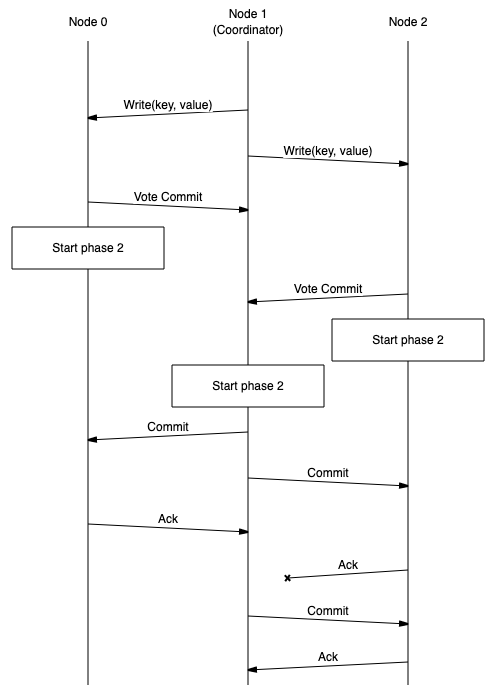
\includegraphics[width=0.75\linewidth]{figs/2pc.png}}
\caption{A two-phase commit between 3 nodes.}
\label{2pc}
\end{figure}

2PC is used to provide atomicity in write transactions. The quorum assembly algorithm requires that every write is written to at least $W$ nodes. 2PC ensures that, once $W$ nodes have been assembled, a value is written to either all of them or none of them, and no conflicting transactions can be interleaved at a time when the value has been written at some nodes but not at all of them.

As its name suggest, two-phase commit involves 2 phases. In the first phase, each node involved votes on whether the transaction should be committed or aborted. Before voting to commit, a node must write the transaction to persistent storage, so that, should it crash before the transaction is committed, it can recover and resume the transaction.

After a node has voted to commit, it enters the second phase. During this phase, all nodes involved are locked. This enforces mutual exclusion, which guarantees serialisability of transactions. Importantly, even if a node crashes, it remains locked until the transaction is completed.

In the second phase, the coordinator sends either a commit instruction or an abort instruction to each node (sending the same instruction to every node). On receipt of either instruction, each node must follow the instruction before releasing its lock.

In the first phase, the coordinator is responsible for collecting votes. It enters its second phase after all other nodes have responded. If all nodes voted to commit, it broadcasts a commit instruction. Otherwise, it broadcasts an abort instruction.

In either case, the coordinator must wait for all nodes to acknowledge that they have completed phase 2, repeating requests if required. Requiring all nodes to acknowledge ensures that all nodes complete the transaction, avoiding leaking locks, which would affect availability.

2PC has some important limitations:

\begin{itemize}
\item
If a node suffers from media failure, a node may fail then recover, but not continue a 2PC transaction. The chance of this can be minimised with robust storage such as RAID, to minimise the risk of data loss and particularly minimise the risk of undetected data loss.

\item
If a node fails permanently, this may block the system until the system is manually un-jammed. This can be mitigated with fine-grained locking and isolated services, to minimise the impact on applications.

\item
A node which fails then recovers can block the system for some time, impacting availability during that time.

\end{itemize}

\section{Sloppy Quorum}

My sloppy quorum system is a modification to the strict quorum system, which provides eventual consistency and the consistent prefix guarantee. The procedure for transactions is the same as before, but without the constraint $R + W > N$.

This means that a read transaction may not return the most recent value for the requested key; it may return a stale value. The benefit is that more read transactions can occur concurrently, which allows a greater throughput of transactions, and the system can remain available for reads when a large number of nodes are unreachable: as long as at least $R$ nodes can be reached, read transactions can still occur.

In an eventually consistent system, if there are no write transactions, the whole system should reach a strongly consistent state after some amount of time. This means that every read transaction should eventually return the most recently written value for each key. Having removed the constraint on $R$, this means that values eventually need to be written to at least $N - R + 1$ nodes.

My system achieves this with a background write propagation mechanism. Each write transaction has a coordinator, responsible for committing a write to $W$ nodes. This coordinator is also responsible for ensuring the write eventually reaches $N - R + 1$ nodes. My system assumes that the set of nodes is fixed, and there is no requirement for the time to reach consistency, so the coordinator can resume this task after failure and recovery without issue.

Once a write transaction has been committed, the coordinator knows the set of nodes which have received the new value. The coordinator is responsible for increasing that set until its size is at least $N - R + 1$, or it becomes aware of a more recent write to the same key.

The coordinator sends lightweight write requests to other nodes, with its new value. These are distinct from full write transactions with 2PC; each one involves only 2 nodes, the coordinator and the node receiving the request. When a node receives a lightweight write request, it should check the value it has stored for that key (if any).

If it has a newer value stored (higher timestamp), it returns the newer value to the coordinator. The coordinator, on receipt of this, updates its own store, and stops propagating its own older value.

If it has an older value stored, it writes the new value and timestamp. If the value is stored successfully, it responds to the coordinator. On receipt of this, the coordinator can add the node to its set of nodes known to have the value. if the size of the set has reached the threshold, the coordinator can stop propagating the write.

If the coordinator receives no response from a node, it just continues retrying. In order to guarantee eventual consistencyeventual consistcy the coordinator must continue retrying indefinitely until it reaches a termination condition.

\section{Leadership Election}

With $N$ nodes, my system constrains the write quorum size $W$ with $W > N / 2$. This means that there can never be concurrent writes; if two nodes each simultaneously attempt to assemble a quorum for a write transaction, they cannot both succeed at the same time. This means there has to be a mechanism to avoid a deadlock condition. I implemented a timeout, which aborts a transaction if assembling a quorum takes too much time; one of the conditions for deadlock is no preemption, so a deadlock cannot occur.

While this recovers from the deadlock, usually both transactions fail in this case, and often a large number of nodes are locked until the transactions are aborted. This has a significant effect on the system's throughput. My system allows any database node to receive client requests and coordinate transactions. Since attempted concurrent writes are expensive, I built a mechanism to minimise the number of instances when this occurs. This is based on a ring election algorithm.

The idea is, since there cannot be concurrent writes, make a single node responsible for coordinating all write transactions. Rather than rely on a single node (and be unavailable for writes when the node is unreachable), a node is elected. Note that attempted concurrent writes affect performance rather than correctness, so my system can tolerate no consensus on the current leader (different nodes disagree on the current leader), although this should be avoided.

All nodes are considered part of a virtual ring. This is defined based on node IDs, since these are assigned sequentially. If there are $N$ nodes in total, 2 nodes $a$ and $b$ are adjacent in the ring if $a-b \equiv 1 \bmod N$ or $b-a \equiv 1 \bmod N$.

There is a token message continually forwarded around the ring, containing a list of node IDs. When each node receives the token, it does the following:

\begin{itemize}
\item
Send an acknowledge (ACK) message to the sender (the previous node in the ring).

\item
Add its own ID to the token, if not already present.

\item
Pick the current leader as the highest ID listed in the token, updating its local record of the leader ID.

\item
Forward the token to the next node in the ring.

\item
If no ACK is received after a timeout, remove the next node's ID from the token (if present), and forward the token to the node after next. This procedure is applied recursively so that, as long as at least one other node is available, a node will always forward the token to the next reachable node in the ring.

\end{itemize}

This means that an unreachable node will be detected by all nodes after at most the time taken for the token to traverse the ring, plus the timeout length.

The token may be lost, if a node fails before forwarding it. To fix this, any node which does not receive the token for some time should create a new token. Until a new token has traversed the ring, nodes will disagree on the current leader, but will reach consensus after one traversal (unless the token is lost again). This is acceptable for my system.

Since any node may create a token, the system may reach a state when there are many tokens. This is not a problem, but should be avoided. To fix this, each node has a rate-limiter, enforcing a minimum time between forwarding 2 tokens. Any tokens to be sent before the minimum time has elapsed are discarded, limiting the total number of tokens in use.

I tested my system with and without the leadership election. Each test uses strict quorum with 5 nodes, with read and write quorum sizes both 3. The system was sent 100 requests per second (figure~\ref{electorhist}).

\begin{figure}[ht]
\centerline{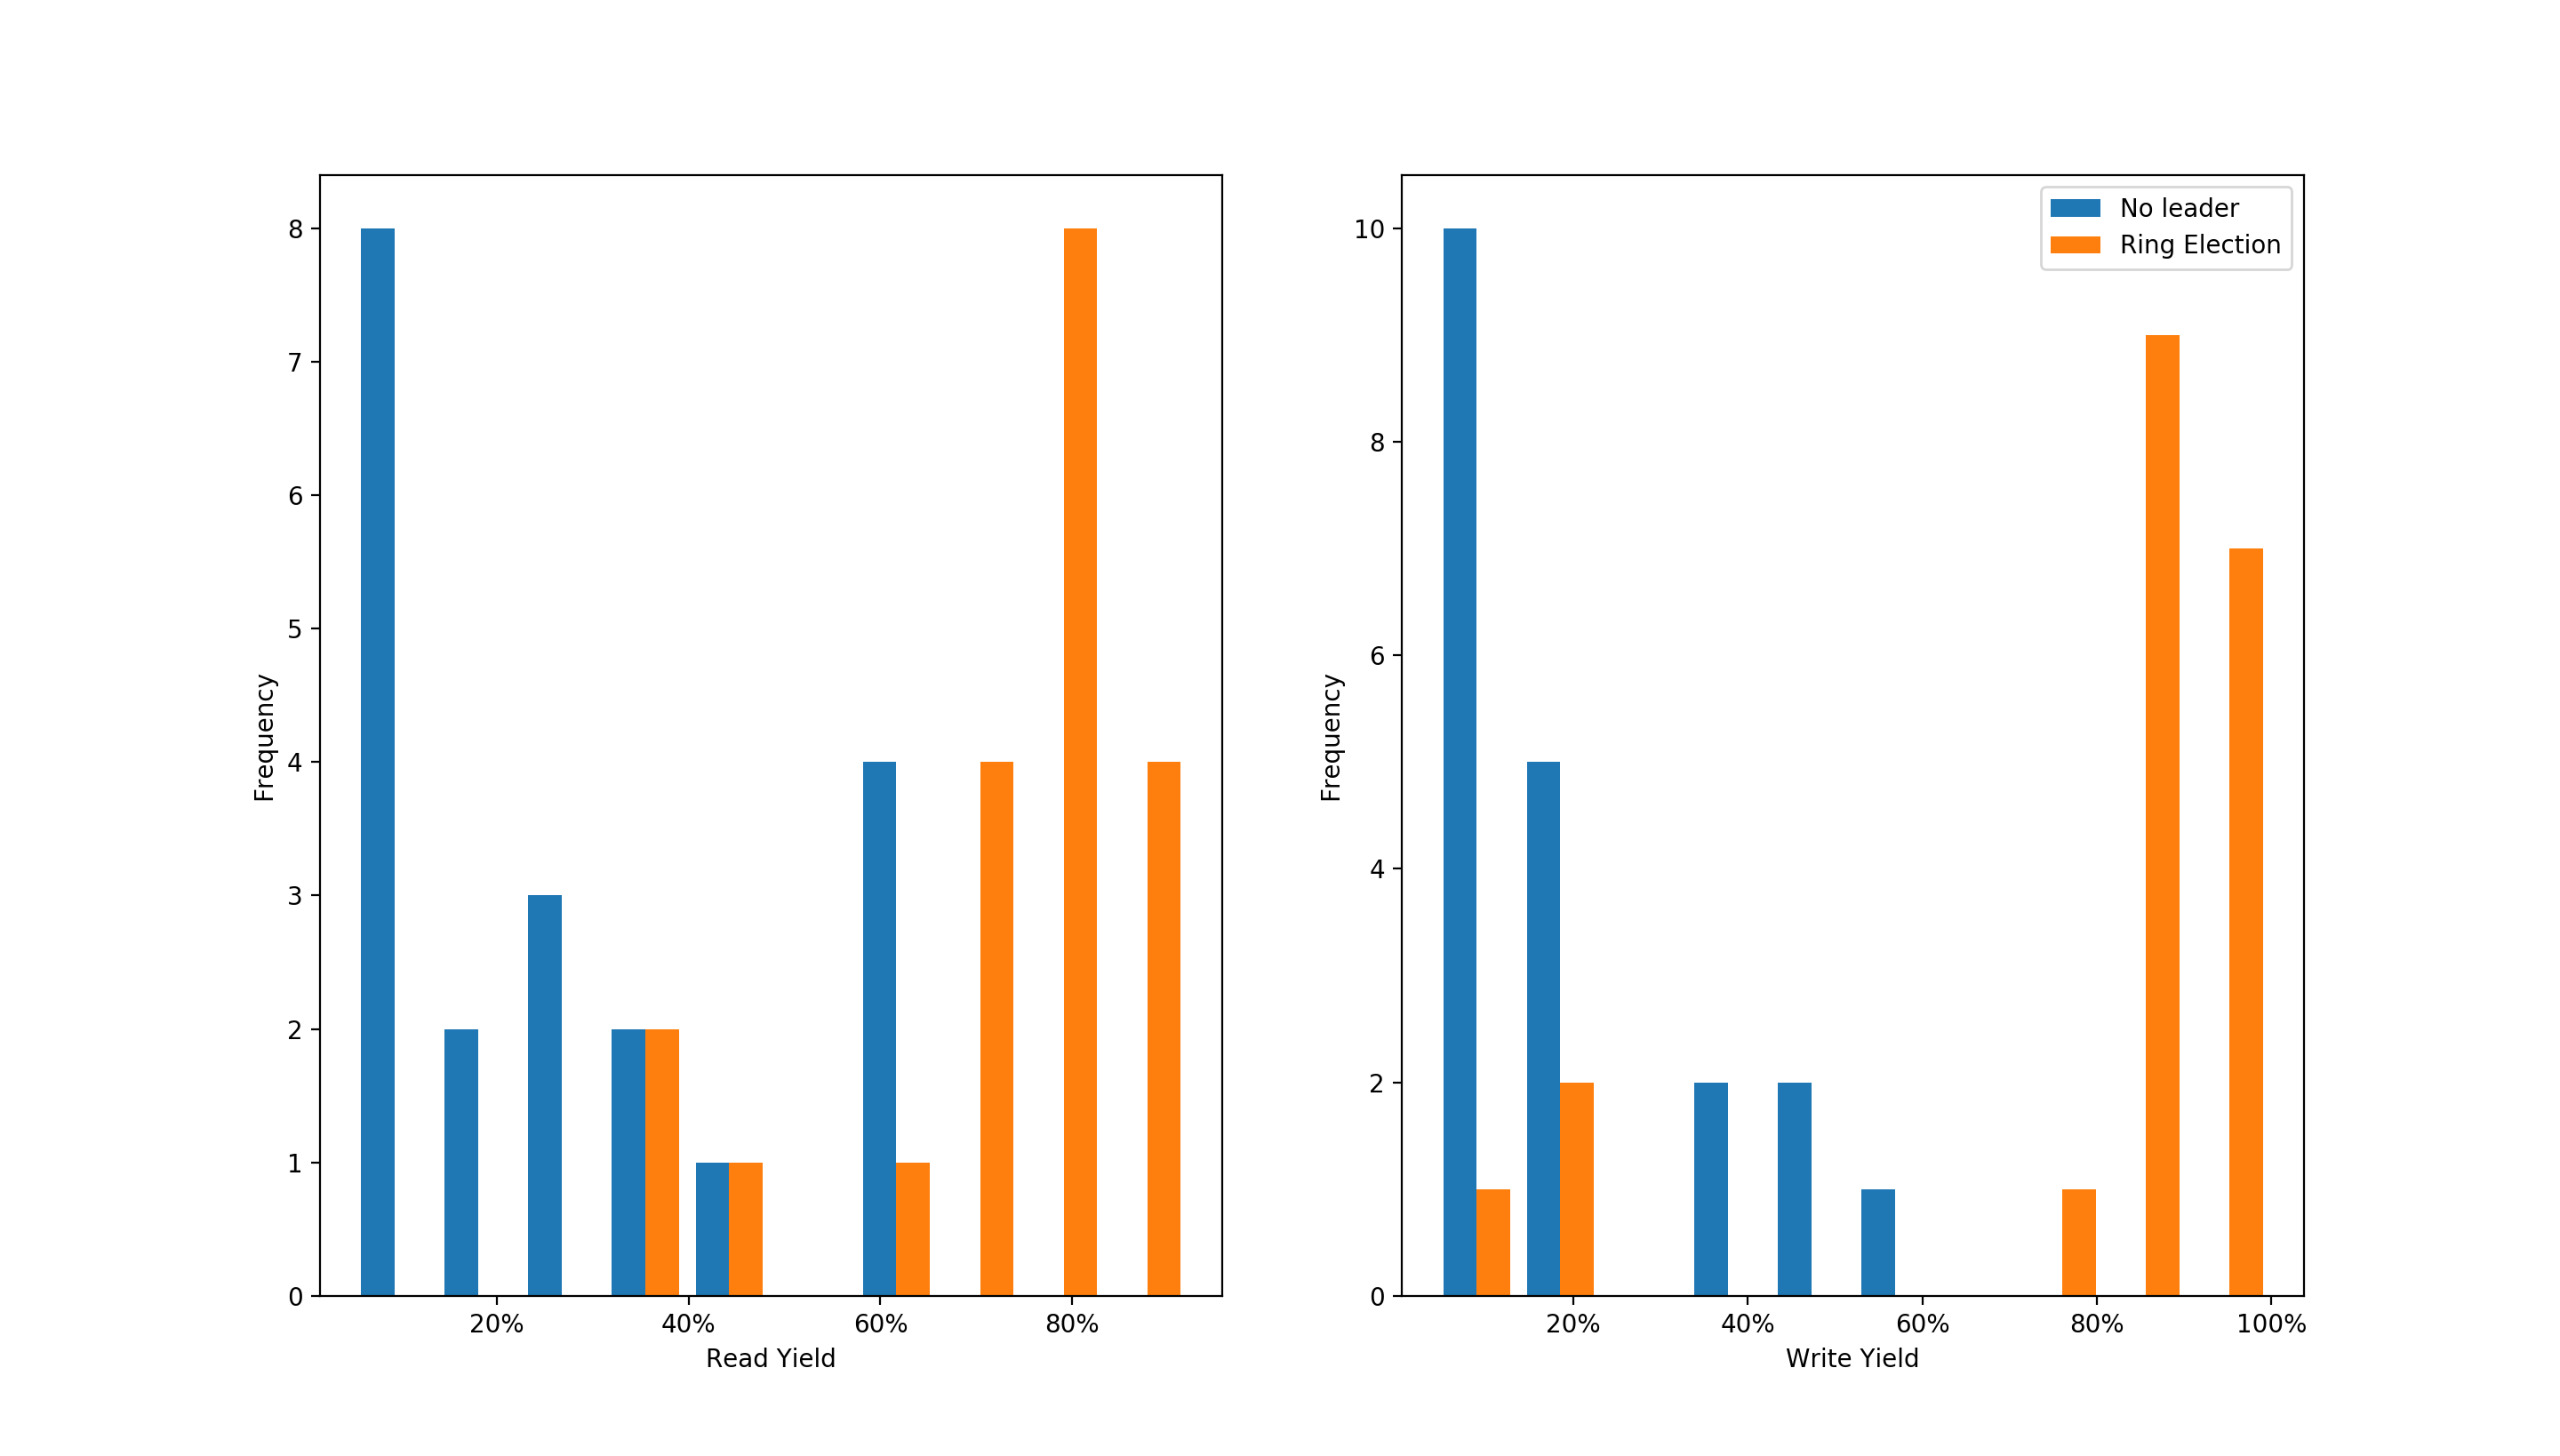
\includegraphics[width=\linewidth]{figs/elector-hist.png}}
\caption[Read and write yield in tests comparing my system with and without a leadership election]{Distribution of read and write yield among 20 tests with a ring election and 20 tests without a leader. Each test uses 5 database nodes, with read and write quorum sizes both equal to 3. Yield is the proportion of transactions which are successful.}
\label{electorhist}
\end{figure}

The write yield (proportion of write transactions which are successful) is higher with a ring election (mean $77.2\%$) than without a leader (mean $22.4\%$), based on 20 repeats of each case (Wilcoxon rank-sum, $p < 0.001$). The chance of 2 nodes racing to assemble quorums is far smaller.

The read yield is also higher with an election ($86.9\%$, compared to $14.3\%$, Wilcoxon rank-sum, $p < 0.001$), since nodes waste far less time attempting (and failing) to coordinate writes.

\begin{table}[ht!]
\centering
\renewcommand{\arraystretch}{1.3}
\begin{tabular}{@{} l l l l l @{}}
\toprule
& \multicolumn{2}{c}{\bf Latency of Reads (ms)} & \multicolumn{2}{c}{\bf Latency of Writes (ms)} \\
\cmidrule(lr){2-3}
\cmidrule(lr){4-5}
& Median & 99th Percentile & Median & 99th Percentile \\
\hline
No Leader & 260 & 521 & 597 & 3131 \\
Ring Election & 63 & 503 & 339 & 4558 \\
\bottomrule
\end{tabular}
\caption[Latency in tests comparing my system with and without a leadership election]{Latency of successful read and write transactions with and without a leader. Each test uses 5 database nodes, with read and write quorum sizes both equal to 3.}
\label{electorlatency}
\end{table}

The median latency is shorter with a single leader (table~\ref{electorlatency}). Without a single leader, when a lock is requested, that lock may be held by another coordinator. This means the lock operation will block. The write cannot proceed until all locks have been acquired. With a single leader coordinating all writes, at the lock acquisition stage, there can be no locks currently held by other transactions, so latency is reduced.

The 99th percentile latency is longer because more transactions are successful. Write transactions involve two-phase commit, which is a blocking protocol. This means that some write transactions have very long latency, in the presence of network unreliability. Without a leader, each write transaction is more likely to fail, especially in the presence of failures (several coordinators racing to lock fewer available nodes). Using a leader, the transactions most likely to fail are more likely to succeed (as shown in the yield test), but with increased latency. 
\section{Thread Confinement}

My database system, like all distributed systems, uses a lot of concurrency, both between separate database nodes and clients, and within each node. Building concurrency systems requires a lot of work to ensure thread-safety.

My system is built in Go, which provides some helpful primitives for concurrent programming: goroutines and channels.

Goroutines are similar to threads. Rather than using OS-level scheduling, the Go runtime has its own scheduler. Goroutines, unlike normal threads, have dynamically-sized stacks.

Typically, threads have a stack size around 1MB. This means that the number of active threads is limited by memory usage. Using a smaller stack allows more threads, but limits the number of stack frames before a stack overflow error. Using dynamically-sized stacks, the number of active goroutines can be much larger.

Channels in Go are essentially thread-safe queue structures. These are ideal for producer-consumer patterns. Enqueue operations on a channel block if the channel is full, and dequeue operations block if the channel is empty.

Within each database node, my system uses a thread confinement pattern to avoid deadlock and race conditions. This is based on a Go idiom: ``Do not communicate by sharing memory; instead, share memory by communicating.'' \cite{effective} The state of each node belongs to a single goroutine, and cannot be read or modified directly by any other goroutine.

Each database node essentially receives messages from the network, and processes them. How it responds to a message depends on a state machine. Based on this, it may send messages to other nodes or clients, change state and modify its local data store (or several or node of those). Importantly, some operations, such as accessing the data store, require waiting for I/O.

The node's local state machine is owned by a single goroutine responsible for the main loop. This loop must not block for a prolonged period time. Other goroutines within the node are responsible for blocking operations, including setting timers. When a transaction times out, for example, the goroutine responsible cannot update the main state machine; instead, it sends a message to the main loop, using a channel. The main loop receives the message and responds appropriately. Importantly, only the main loop can access the state machine, so there can be no race conditions, without using any locks. Care must be taken to ensure the main loop cannot block, but I found this easier in practice than micro-managing locks (as was necessary in early versions of my implementation).

\section{Out-of-Order Delivery}

Any message sent over a network has some unknown and unbounded latency (really unbounded \cite{imbriaco_2012}). This means that messages may be delivered out-of-order: if a node $A$ sends several messages to node $B$, the order in which they are sent is not always the order in which they arrive. This can cause difficult problems.

What if a node is sent a lock request, then an unlock request very soon after?

If the unlock arrives before the lock, the node may become locked forever.

To fix this, each node stores all transaction IDs for which it has received an unlock request. If it subsequently receives a lock request with an already-seen ID, ignore it.

This leads to each node accumulating a record of every transaction ever, so make it soft state.

% TODO: more about the session layer? repeating requests?

\section{Test Framework}

[Currently copied from design doc, needs rewriting]

% TODO: rewrite this

My system will be built so that it interfaces closely with my test framework, using my RPC system. This will provide an ideal environment for integration testing and evaluating the system's performance. The architecture is based on two of Go's concurrency primitives: goroutines and channels.

Goroutines are similar to threads. Rather than using OS-level scheduling, the Go runtime has its own scheduler. Goroutines, unlike normal threads, have dynamically-sized stacks, between 8 kB and 1 GB \cite{gosrc}. Typically, threads have a stack size around 1MB. This means that the number of active threads is limited by memory usage. Using a smaller stack allows more threads, but limits the number of stack frames before a stack overflow error. Using dynamically-sized stacks, the number of active goroutines can be much larger.

Goroutines also have more efficient scheduling than threads in the OS. For example, the Go runtime knows which registers are live, so can copy the minimum number of register values, whereas the OS has to assume all registers are live and save the contents of all of them.

Channels in Go are essentially thread-safe queue structures. These are ideal for producer-consumer patterns. Consumers can easily poll the queue, blocking until a value is available. My design uses channels to simulate network links.

Each database node will run as its own goroutine. The system will support a fixed number of nodes, so each node will be identified by a unique integer. These will be assigned sequentially and remain constant, so they can be used as addresses in the simulated network. % TODO: discuss name servers (DNS, alternatives)

For each database node, there will be two channels: one for incoming messages, and one for outgoing messages. A message may be a request from a (simulated) external client, a response to such a request, or a message used to coordinate nodes in the system. A message has 3 fields: source and destination addresses (integers), and a payload, the structure of which depends on the type of message. In order to handle a message, the network simulator only needs to inspect the source and destination addresses.

Supporting each database node, there will be an additional goroutine responsible for delivering its outgoing messages. This will use the following algorithm:

\begin{lstlisting}
while true:
    message = outgoingMessages.poll() // Blocking deque

    // Chance of packet loss, based on a given parameter
    if (uniform random value in range [0,1]) < x:
        continue

    // Random latency
    delay = (normal random value, for given mean and variance)
    sendAfterDelay(message, delay)
\end{lstlisting}

The \verb|sendAfterDelay| method spawns a new goroutine, which sleeps for the given time, then appends the message to the recipient's incoming queue. This means that the main loop will not block, so later messages will be delivered without uncontrolled delay.

The main routine will be responsible for simulating clients. This includes generating requests, sending these requests to random database nodes, and recording responses. For each request, it should record the time from request to response (if a response was received). If a request times out without a response, this should also be recorded.

Once all requests have either timed out or been responded to, the main routine will terminate (thus halting the whole system). By configuring the number and type of tests and recording responses (as well as configuring the network properties, as described above), this can be used for both integration testing and evaluating the system's performance.

% TODO: diagram

\chapter{Evaluation}
% 20% (with conclusions)

\section{Goals}

% TODO: words

At the beginning of the project, I set core and stretch goals. I achieved all of the core goals.

I implemented everything required to achieve my core goals: two different quorum-based systems and a simulated network for testing and evaluation purposes. The next section describes consistency tests, which all passed.

The Remainder of this chapter shows performance measurements. This includes availability (yield), latency, and time for the eventually consistent variant to converge on a consistent state.

I also set stretch goals: optimising my implementation and implementing a third system to provide different consistency guarantees. Chapter 3 describes a leadership election, which provides a significant performance improvement compared to my original design. Due to time constraints, I did not implement a third system.

\section{Consistency Guarantees}

In every test, I tested the output is consistenct with the consistent guarantees it should provide. My strict quorum system should provide strong consistency, and my sloppy quorum system should provide eventual consistency with monotonic writes. Each guarantee is tested separately.

In every test case I have, all the appropriate consistency tests have passed. As designed, where my system cannot provide the required consistency, it sacrifices availability. Systems with this property are useful to applications; an application developer can rely on every consistency guarantee being true, and accept imperfect availability. A system which is nearly always available is much better than one which is nearly always consistent (and may not indicate when it is not consistent).

\subsection{Serialisability}

Serialisability means that each transaction appears to be executed instantaneously, at a unique timestamp. Whenever a value is stored, it is associated with a timestamp. Neither the value nor the timestamp can be updated without also updating the other. The serialisability test requires two invariants:

\begin{itemize}
  \item
  Every successful read transaction returns a value-timestamp pair which was written by a successful write transaction (or the null value and 0 timestamp).

  \item
  For any two successful write transactions modifying the same key, those transactions have unique timestamps.

\end{itemize}

\subsection{Strong Consistency}

Strong consistency requires linearisability \cite{herlihy1990linearizability}. This has 2 parts: serialisability, and ordering guarantees for transactions which are not concurrent.

Every successful transaction has 2 timestamps: a start time (when a client sends a request) and an end time (when the client receives a response). These timestamps are distinct from the Lamport clock timestamps stored in my system. A transaction $T$ happens-before another transaction $U$ ($T \rightarrow U$) if $T$'s end time is earlier than $U$'s start time. This means, for any pair of transactions $A$ and $B$, there are 3 possiblities: $A \rightarrow B$, $B \rightarrow A$, or $A$ and $B$ are concurrent (any other case).

If two transactions are concurrent, linearisability only guarantees serialisability. This is tested as described above.

If a transaction $T$ happens-before another transaction $U$, linearisability also requires that $T$ appears to be executed before $U$. If both transactions read from or write to the same key, the timestamp of $T$ must be no greater than the timestamp of $U$.

\subsection{Eventual Consistency}

Eventual consistency is difficult to test, since it allows an indefinite amount of time to pass before the system converges on a strongly consistent state. A later section shows measurements of convergence time.

\section{Availability Without Failures}

\begin{figure}[ht!]
\centerline{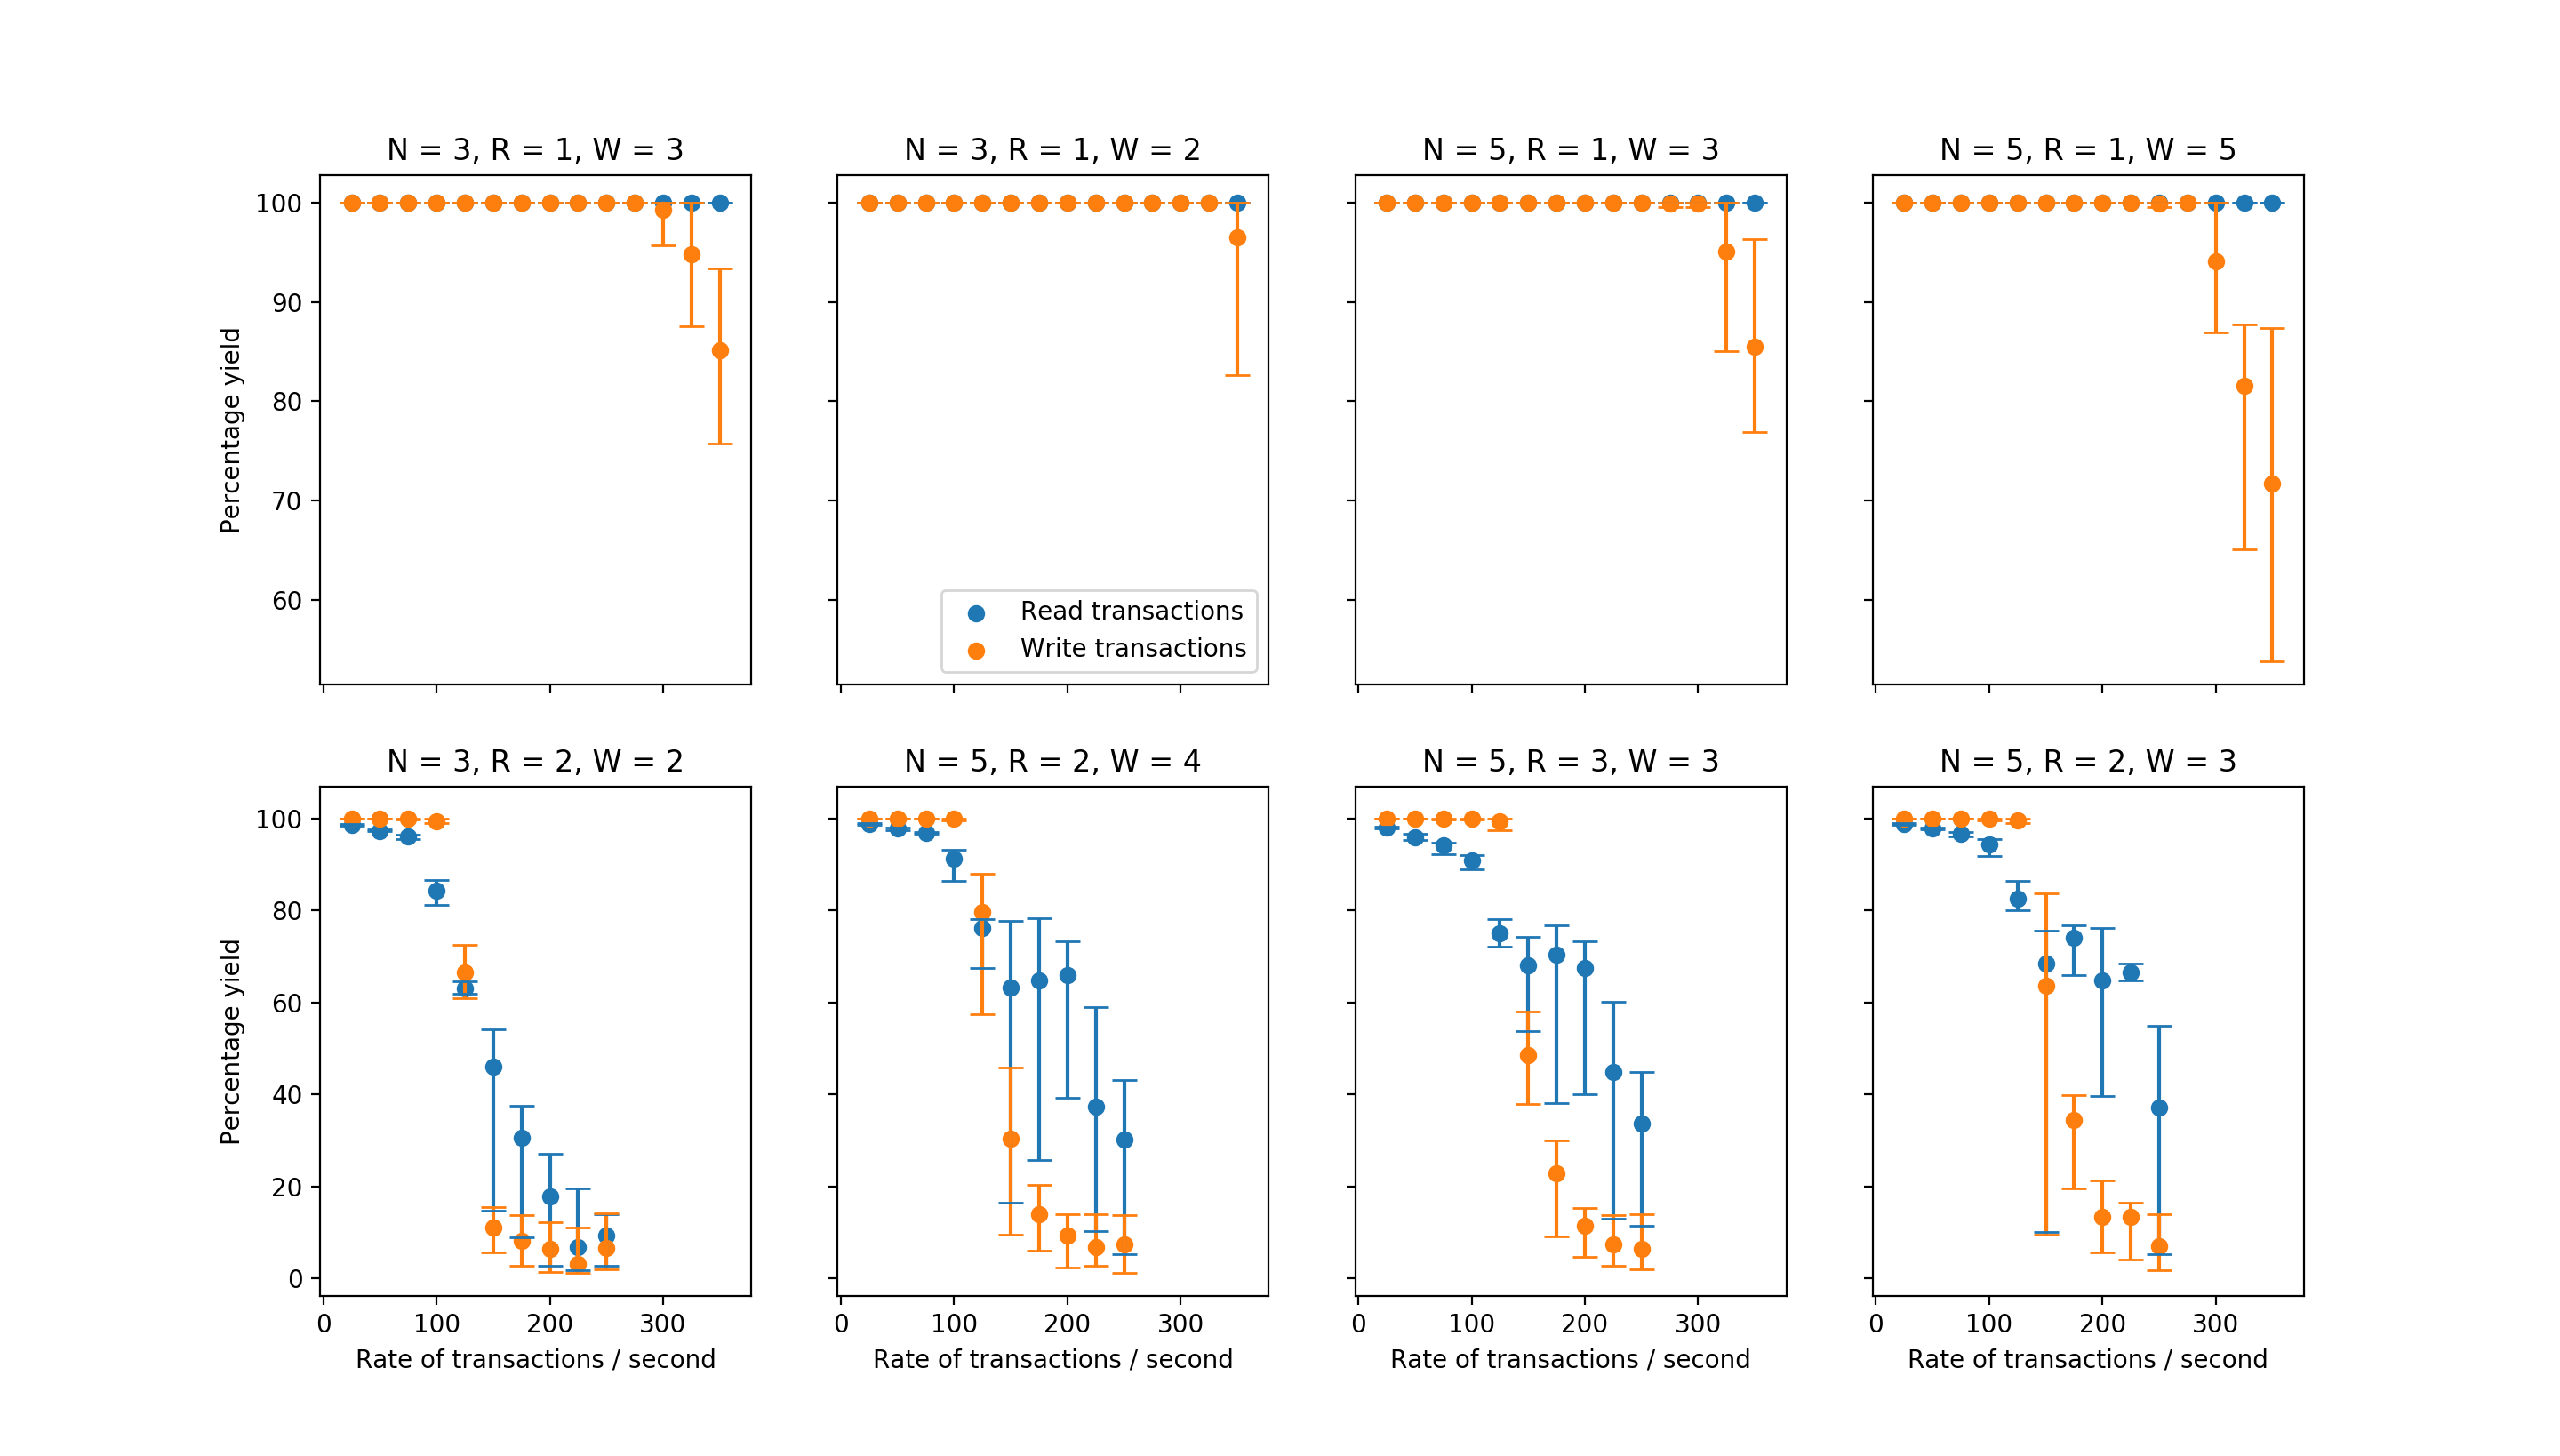
\includegraphics[width=\paperwidth]{figs/eval-fig-1.png}}
\caption[Yield in basic tests with 3 and 5 database nodes, using strict and sloppy quorum]{Yield (proportion of transactions which are successful) in tests with 3 or 5 nodes, without any node or network failures. The rate of requests is varied in each set of tests. The plots show mean values, with error bars showing maximum and minimum.}
\label{yield35nofail}
\end{figure}

I first tested the system without any network or node failures. Every network message is delivered reliably (with variable latency). Each test uses 3 or 5 database nodes ($N \in \{3, 5\}$), with various read and write quorum sizes ($R$ and $W$). Tests with $R + W > N$ use strict quorum, and others use sloppy quorum. Each test involves 10,000 client requests, of which $95\%$ are reads, and is repeated 10 times.

In each test, I measured read and write yield (the proportions of read and write requests which were successfully executed), and latency of successful transactions (time from client request sent to response received by client).

\begin{figure}[ht]
\centerline{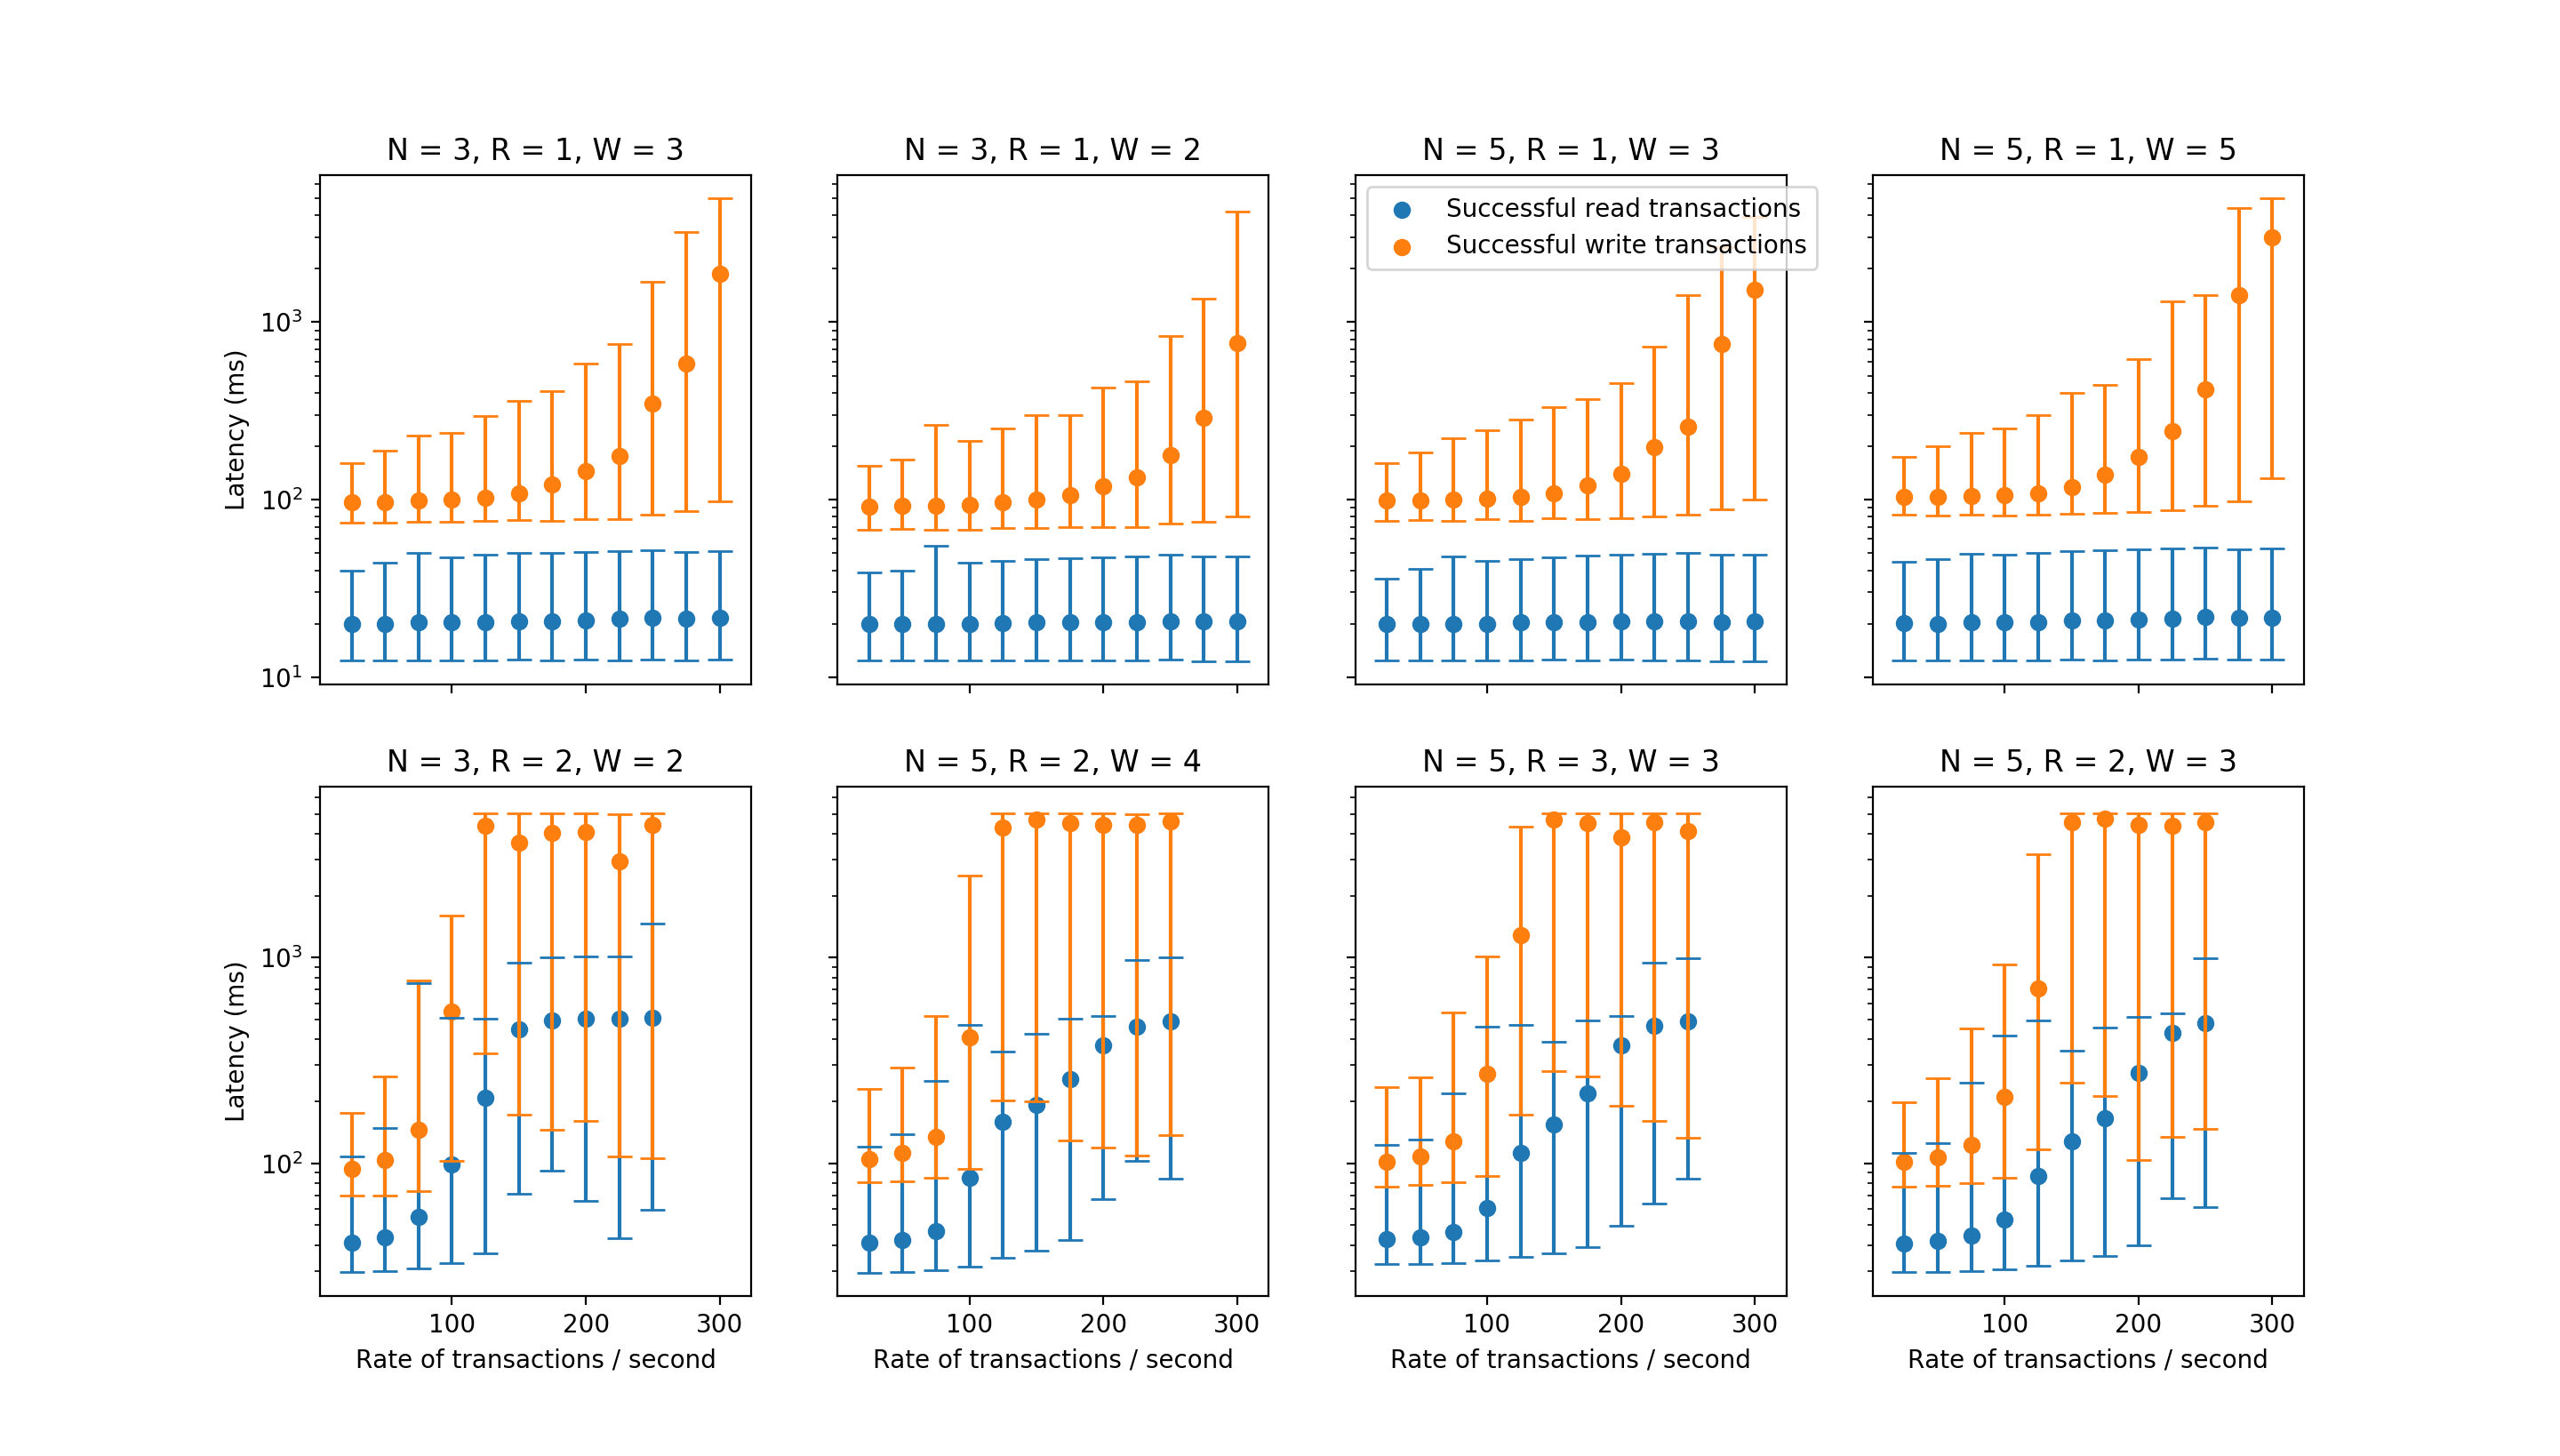
\includegraphics[width=\paperwidth]{figs/eval-fig-5.png}}
\caption{Latency of successful transaction in tests with 3 or 5 nodes, with no node or network failures. Each test is repeated 10 times. The plots show median latencies, with error bars showing 1st and 99th percentiles, plotted on a log-scale.}
\label{latency35nofail}
\end{figure}

Tests with $R = 1$ have much better performance, especially for reads. In every test where $R = 1$, read yield was $100\%$. Whenever a node receives a read request, it can immediately respond without involving any other nodes, then immediately become available for other transactions. With no failures, every request reaches an available node, so every read request succeeds.

Read requests also have lower latency with $R = 1$, and that latency is not affected by varying the rate of transactions. % TODO: a stats test
Reads with $R > 1$ take at least 1 RTT longer than with $R = 1$, as shown in figure~\ref{r1}. In the case when other nodes are busy with other transactions, they take longer to respond. This results in increased latency, and increased chance of failure (so lower yield).

For read-heavy applications, $R = 1$ gives better availability for reads and writes, measured by both yield and latency.

In each set of tests, figure~\ref{yield35nofail} clearly shows the maximum rate at which write yield is higher than $95\%$. This indicates the maximum throughput of the system with each configuration. At higher rates than the maximum throughput, yield declines and latency increases rapidly. % TODO: is this true? why?
This property might be improved by rate-limiting requests; by keeping the rate of requests lower than the maximum throughput, the number of successful transactions is increased. Given the distributed nature of the system, rate-limiting may be difficult to implement; a key benefit of available is the fact that any node can receive requests; adding a simple rate-limiter would introduce a single point-of-failure, negating this advantage.

TODO: statistical tests: does sloppy quorum have better yield? does sloppy quorum have lower latency?

\begin{figure}[ht]
\centerline{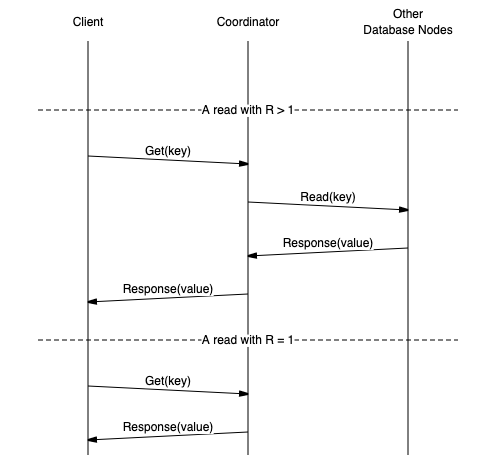
\includegraphics[width=\linewidth]{figs/r1.png}}
\caption{Two read transactions, with different read quorum sizes. Read latency is significantly reduced when the read quorum size ($R$) is 1.}
\label{r1}
\end{figure}

\section{Availability With Failures}

\begin{figure}[ht!]
\centerline{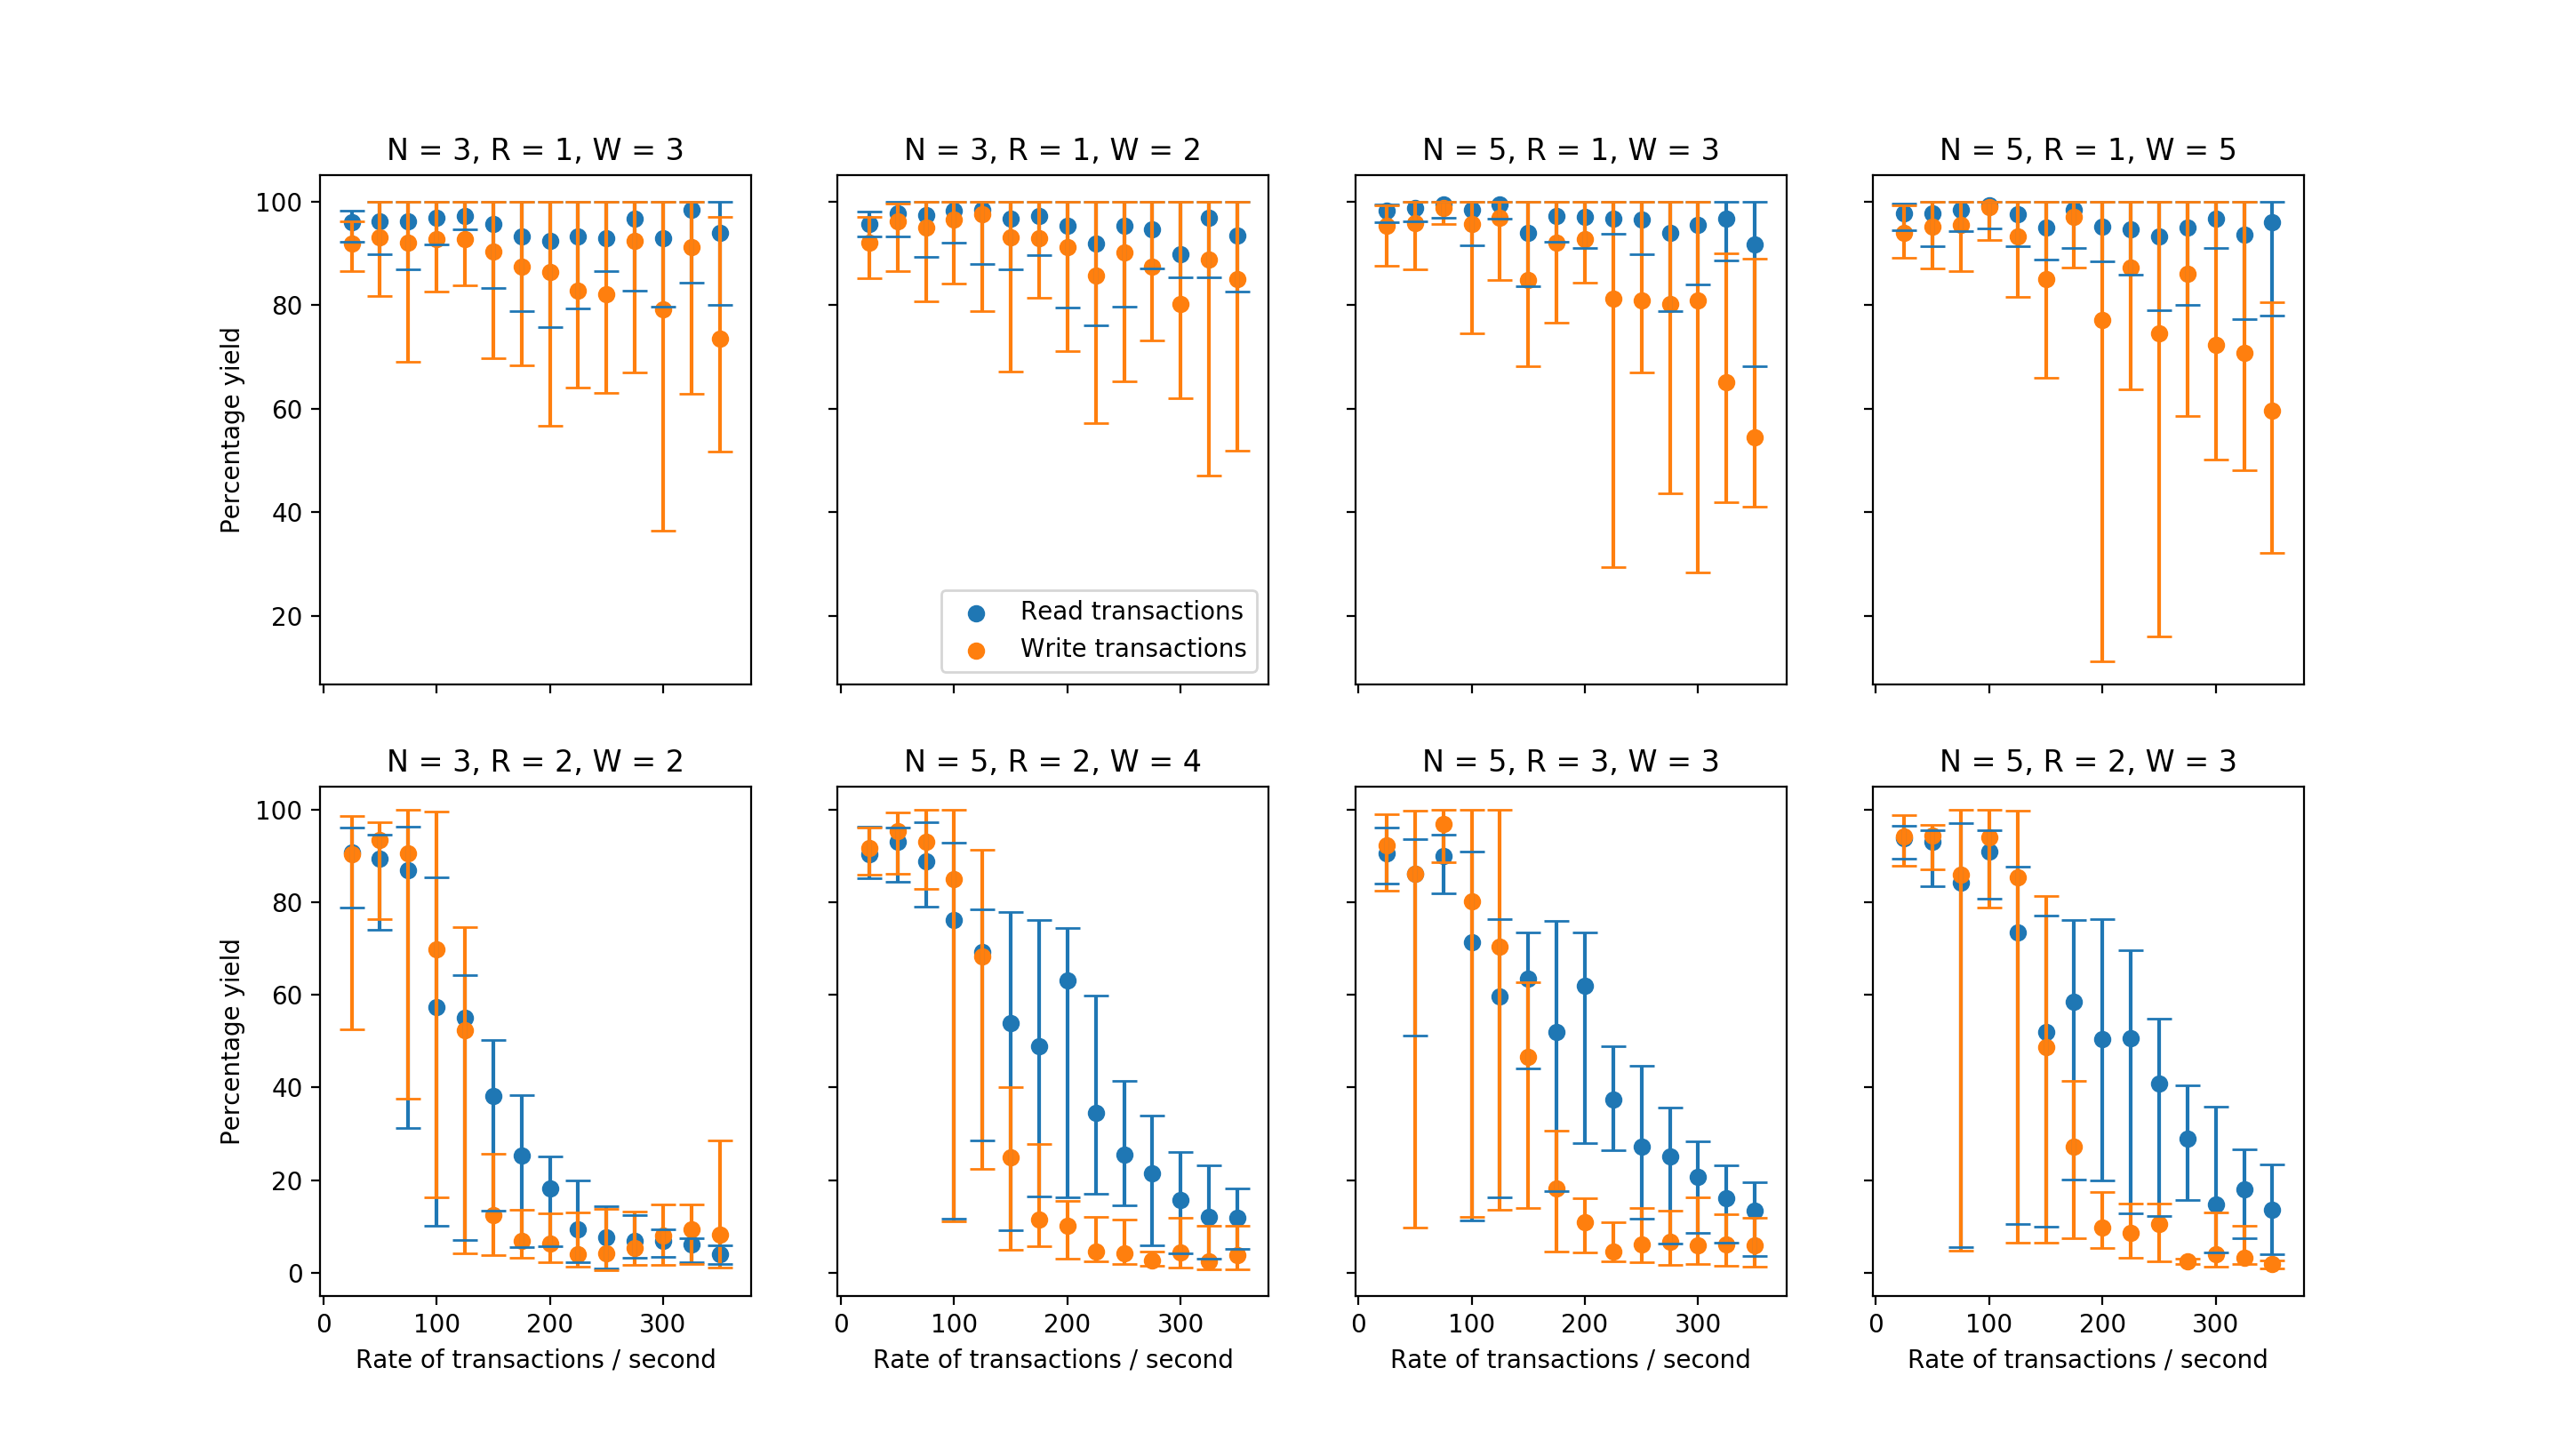
\includegraphics[width=\paperwidth]{figs/eval-fig-2.png}}
\caption{Yield of tests with 3 or 5 nodes, with random node and network failures. Plots show mean from 10 tests, with error bars showing maximum and minimum.}
\label{yield35normal}
\end{figure}

I repeated the tests from the previous section with random node and network failures. Failures are Poisson-distributed, with on average 1 failure per 100 seconds. Each failure is either a node failure (a random node stop responding to requests and loses all non-persistent state), or a partition (a random set of network links stops working). Every failure recovers after a random delay (average 10 seconds).

Yield trends are the same as before, but with much more noise (figure~\ref{yield35normal}).

Next look at particular tests in detail to understand big error bars in both cases. % TODO

\begin{figure}[ht]
\centerline{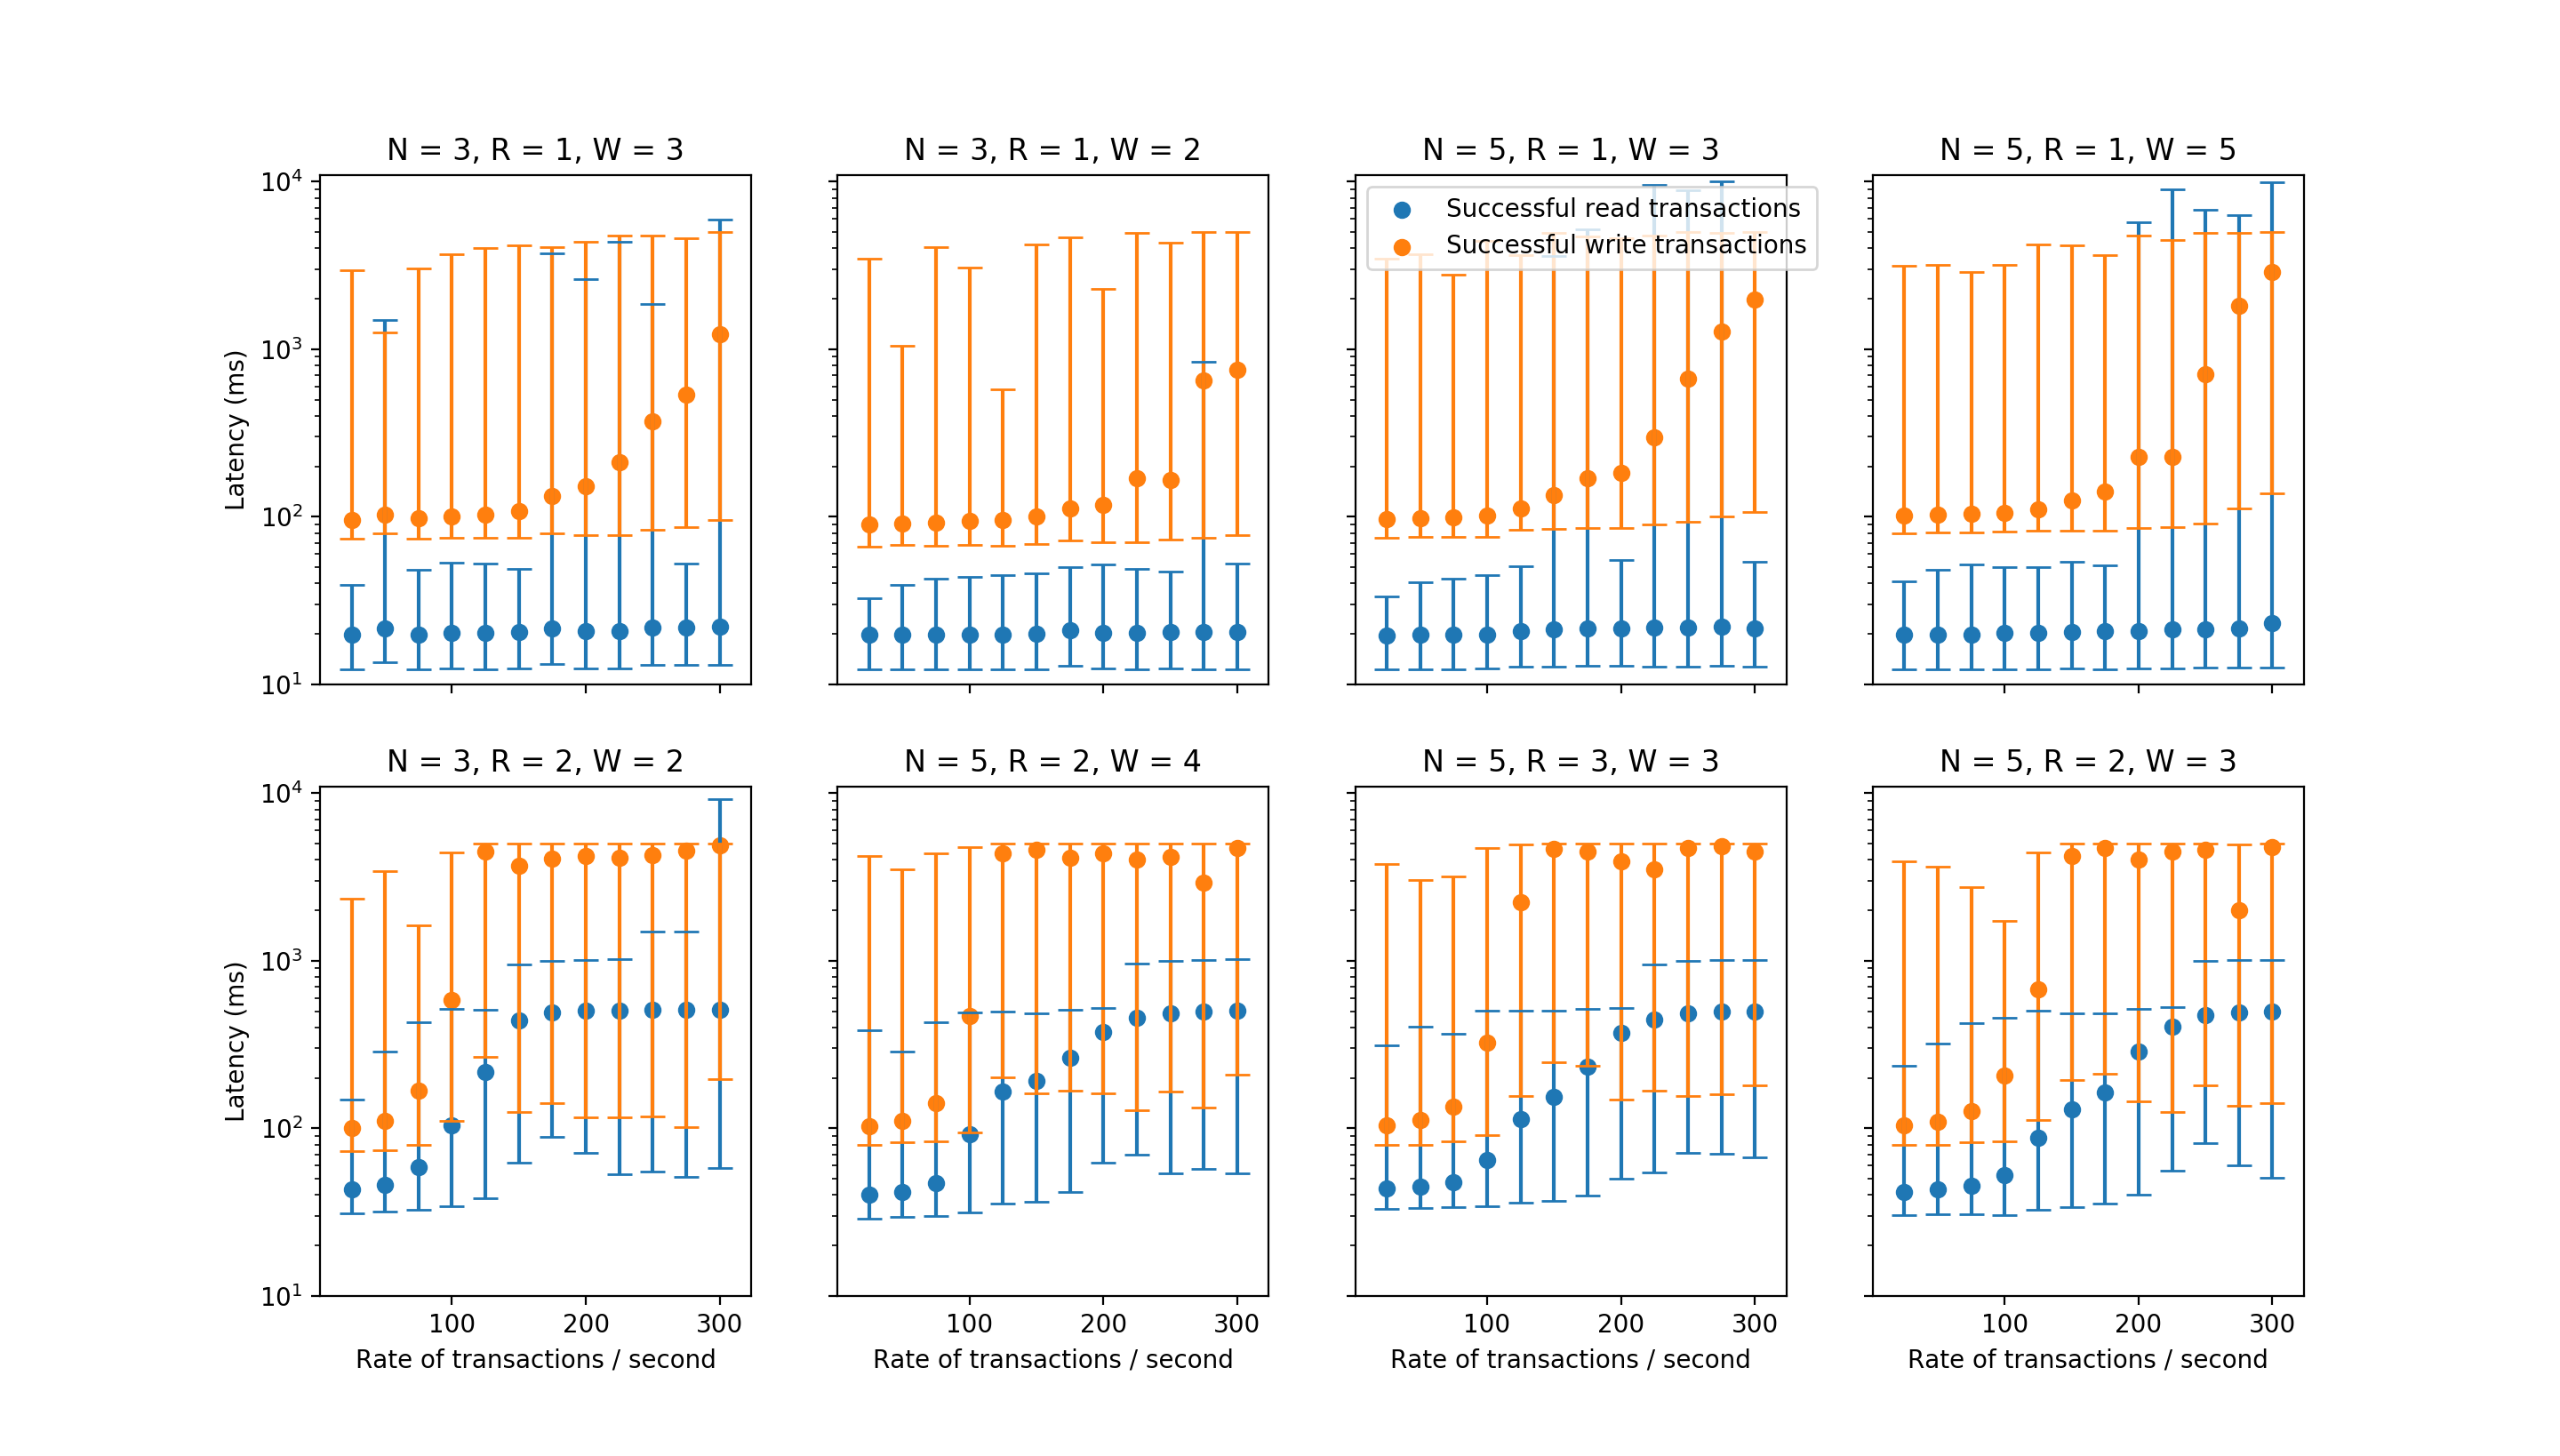
\includegraphics[width=\paperwidth]{figs/eval-fig-6.png}}
\caption{Latency of successful transaction in tests with 3 or 5 nodes, with random node and network failures. Each test is repeated 10 times. The plots show median latencies, with error bars showing 1st and 99th percentiles, plotted on a log-scale.}
\label{latency35normal}
\end{figure}

Mean latency of successful transactions is the same as without failures. % TODO: test
Most of the time, there is no failure.

99th percentile is much higher. % TODO: test
Some write transactions block the system when a failure occurs during 2PC. Other requests sit in queues until after the failure has recovered, resulting in much higher latency.

In general, high latency is undesirable but better than failure. Is there some application which might prefer to fail fast? % TODO

\section{Failure Modes}

\begin{figure}[htb]
% normal/50/5-1-3-2.txt
\centerline{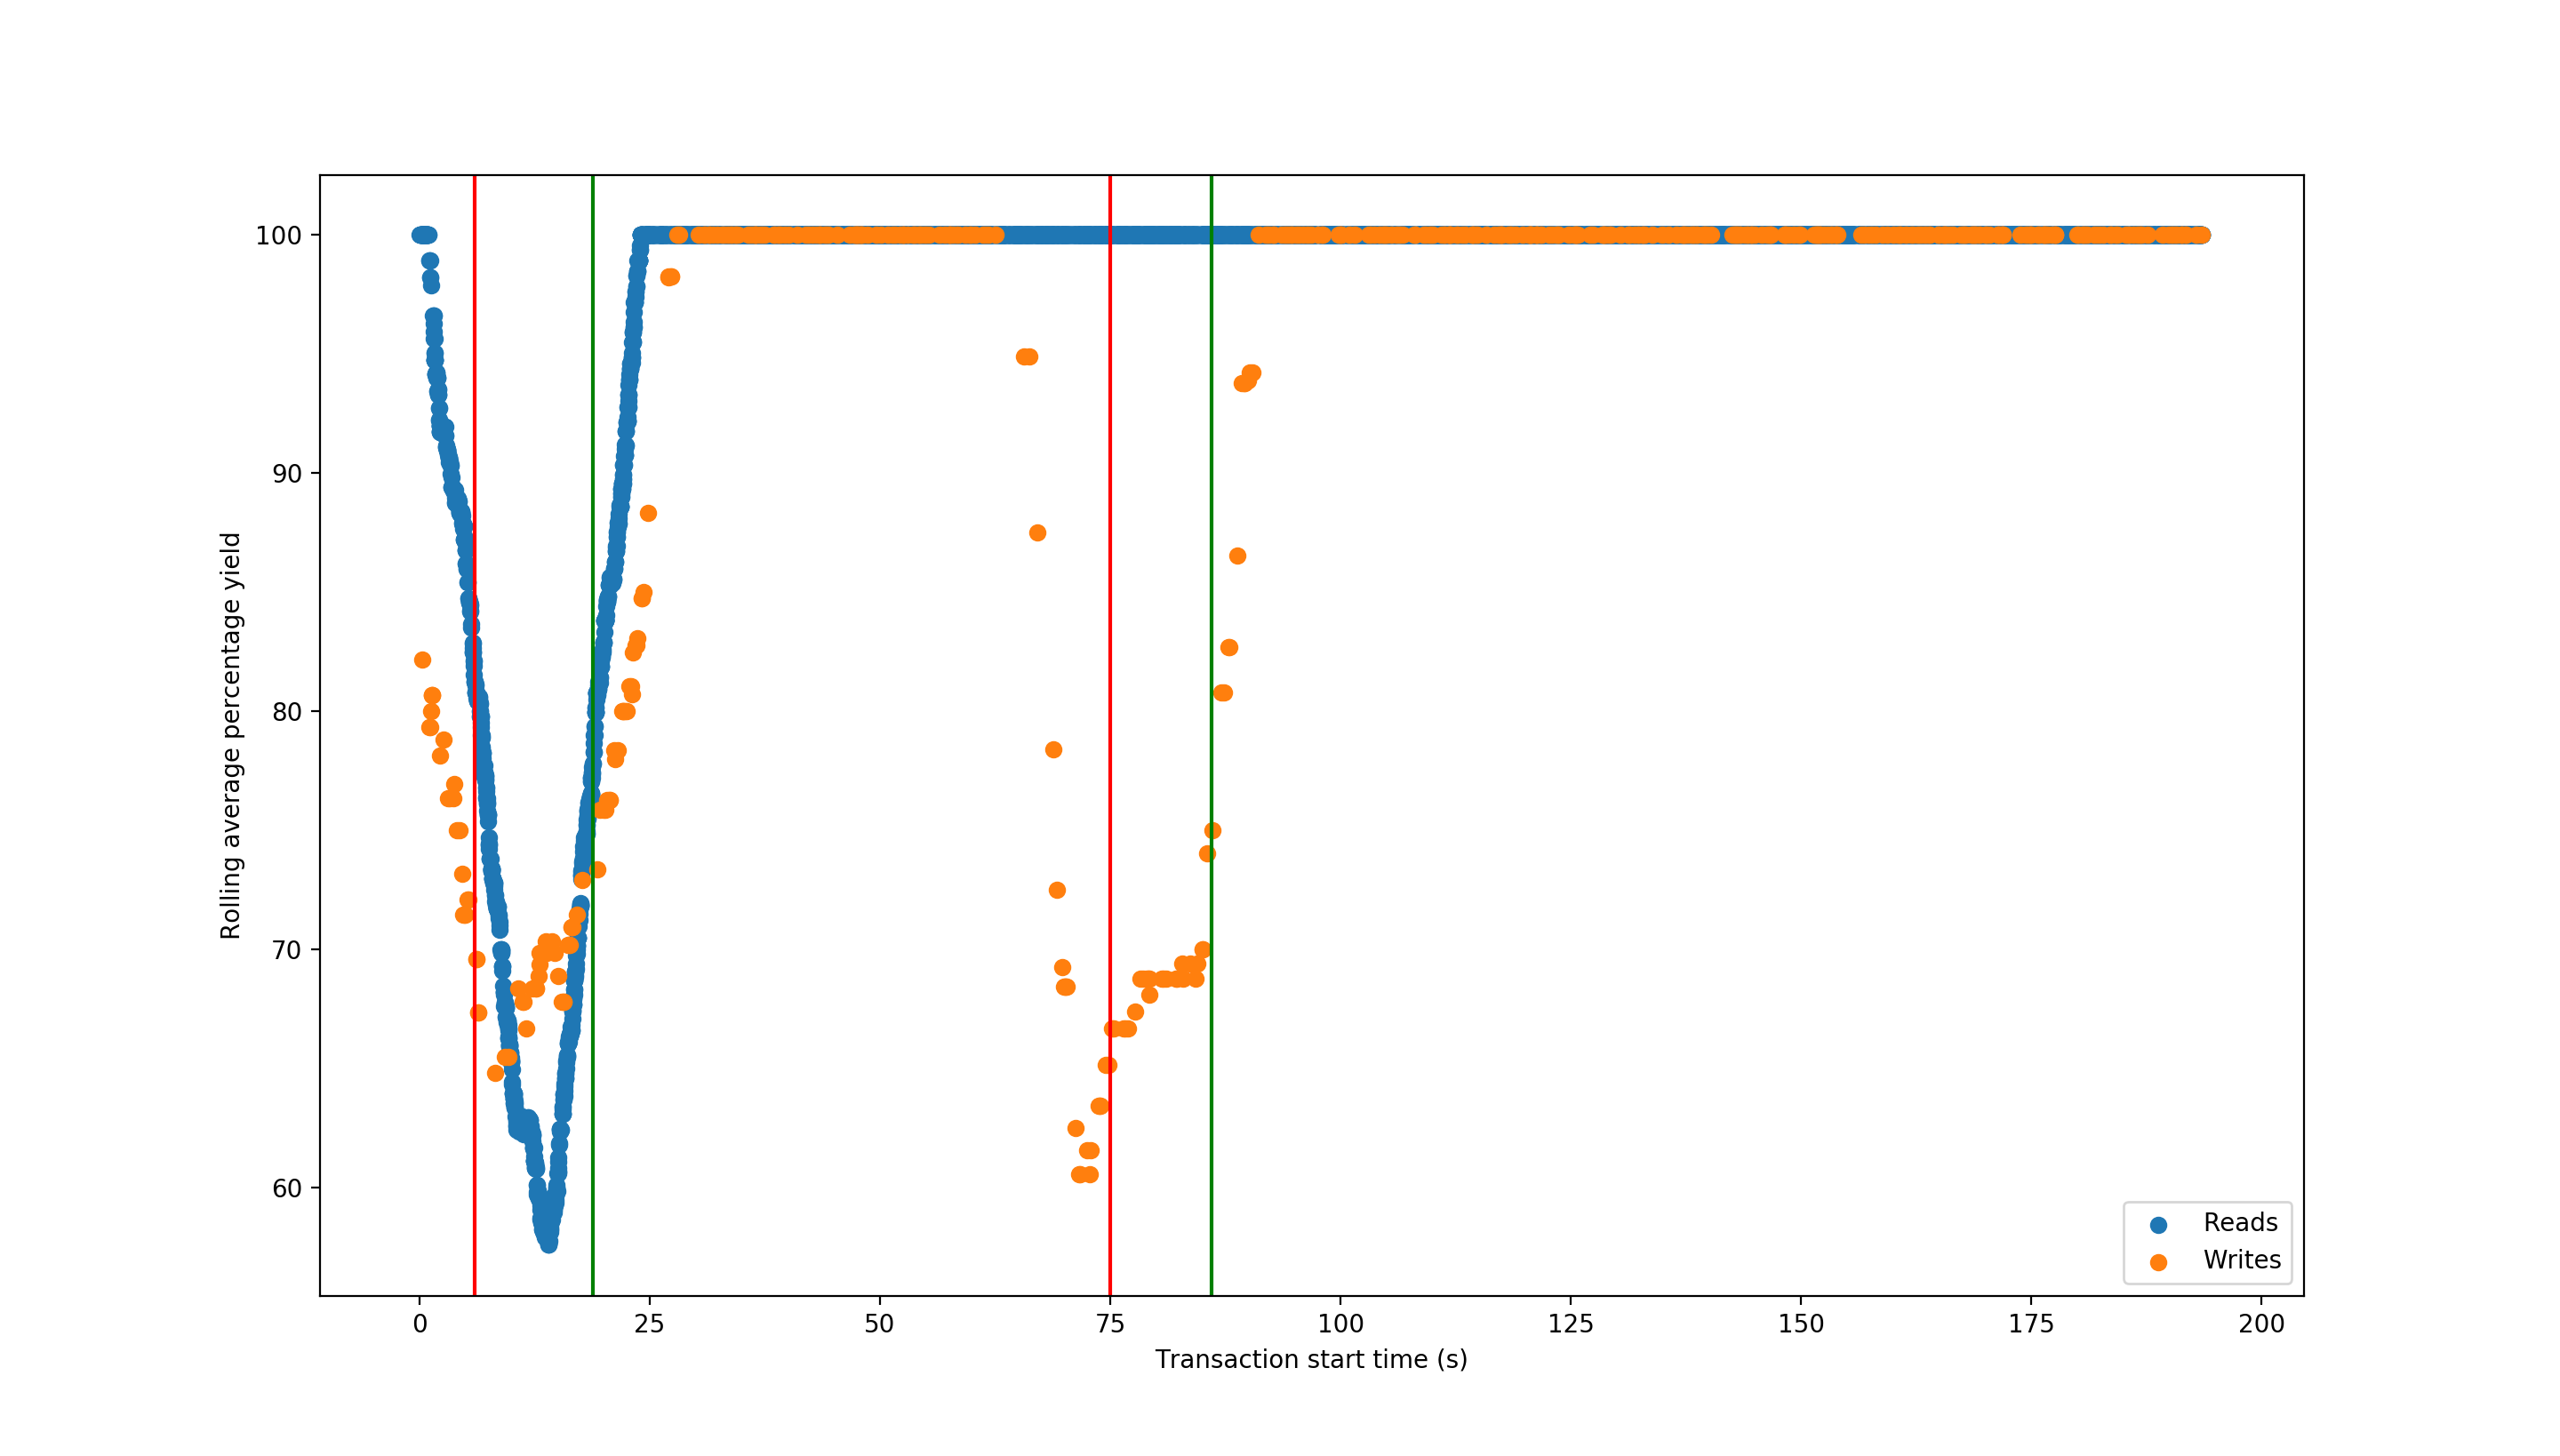
\includegraphics[width=\linewidth]{figs/eval-fig-3.png}}
\caption{Rolling average yield over time for a particular test case, with 5 nodes, read quorum size 1, write quorum size 3. Request rate 50 per second. Red lines indicate network partitions. Green lines indicate partition recoveries.}
\label{single-test-normal}
\end{figure}

When no part of the system has failed, yield is optimal. At low enough transaction rates (depending the on number of nodes and quorum sizes), yield is $100\%$ for both reads and writes. This is shown in figure~\ref{single-test-normal}, alongside yield during partitions. In one partition, yield drops to around $60\%$. With 5 nodes, this indicates that 2 nodes were unreachable by clients (since my system use no load-balancing). In a second partition, read yield remains at $100\%$. This indicates that all nodes are reachable by clients. With read quorum size 1, only a single node is involved in each read. Write yield is much lower, indicating that, in some case, nodes failed to assemble quorums.

\begin{figure}[htb]
\centerline{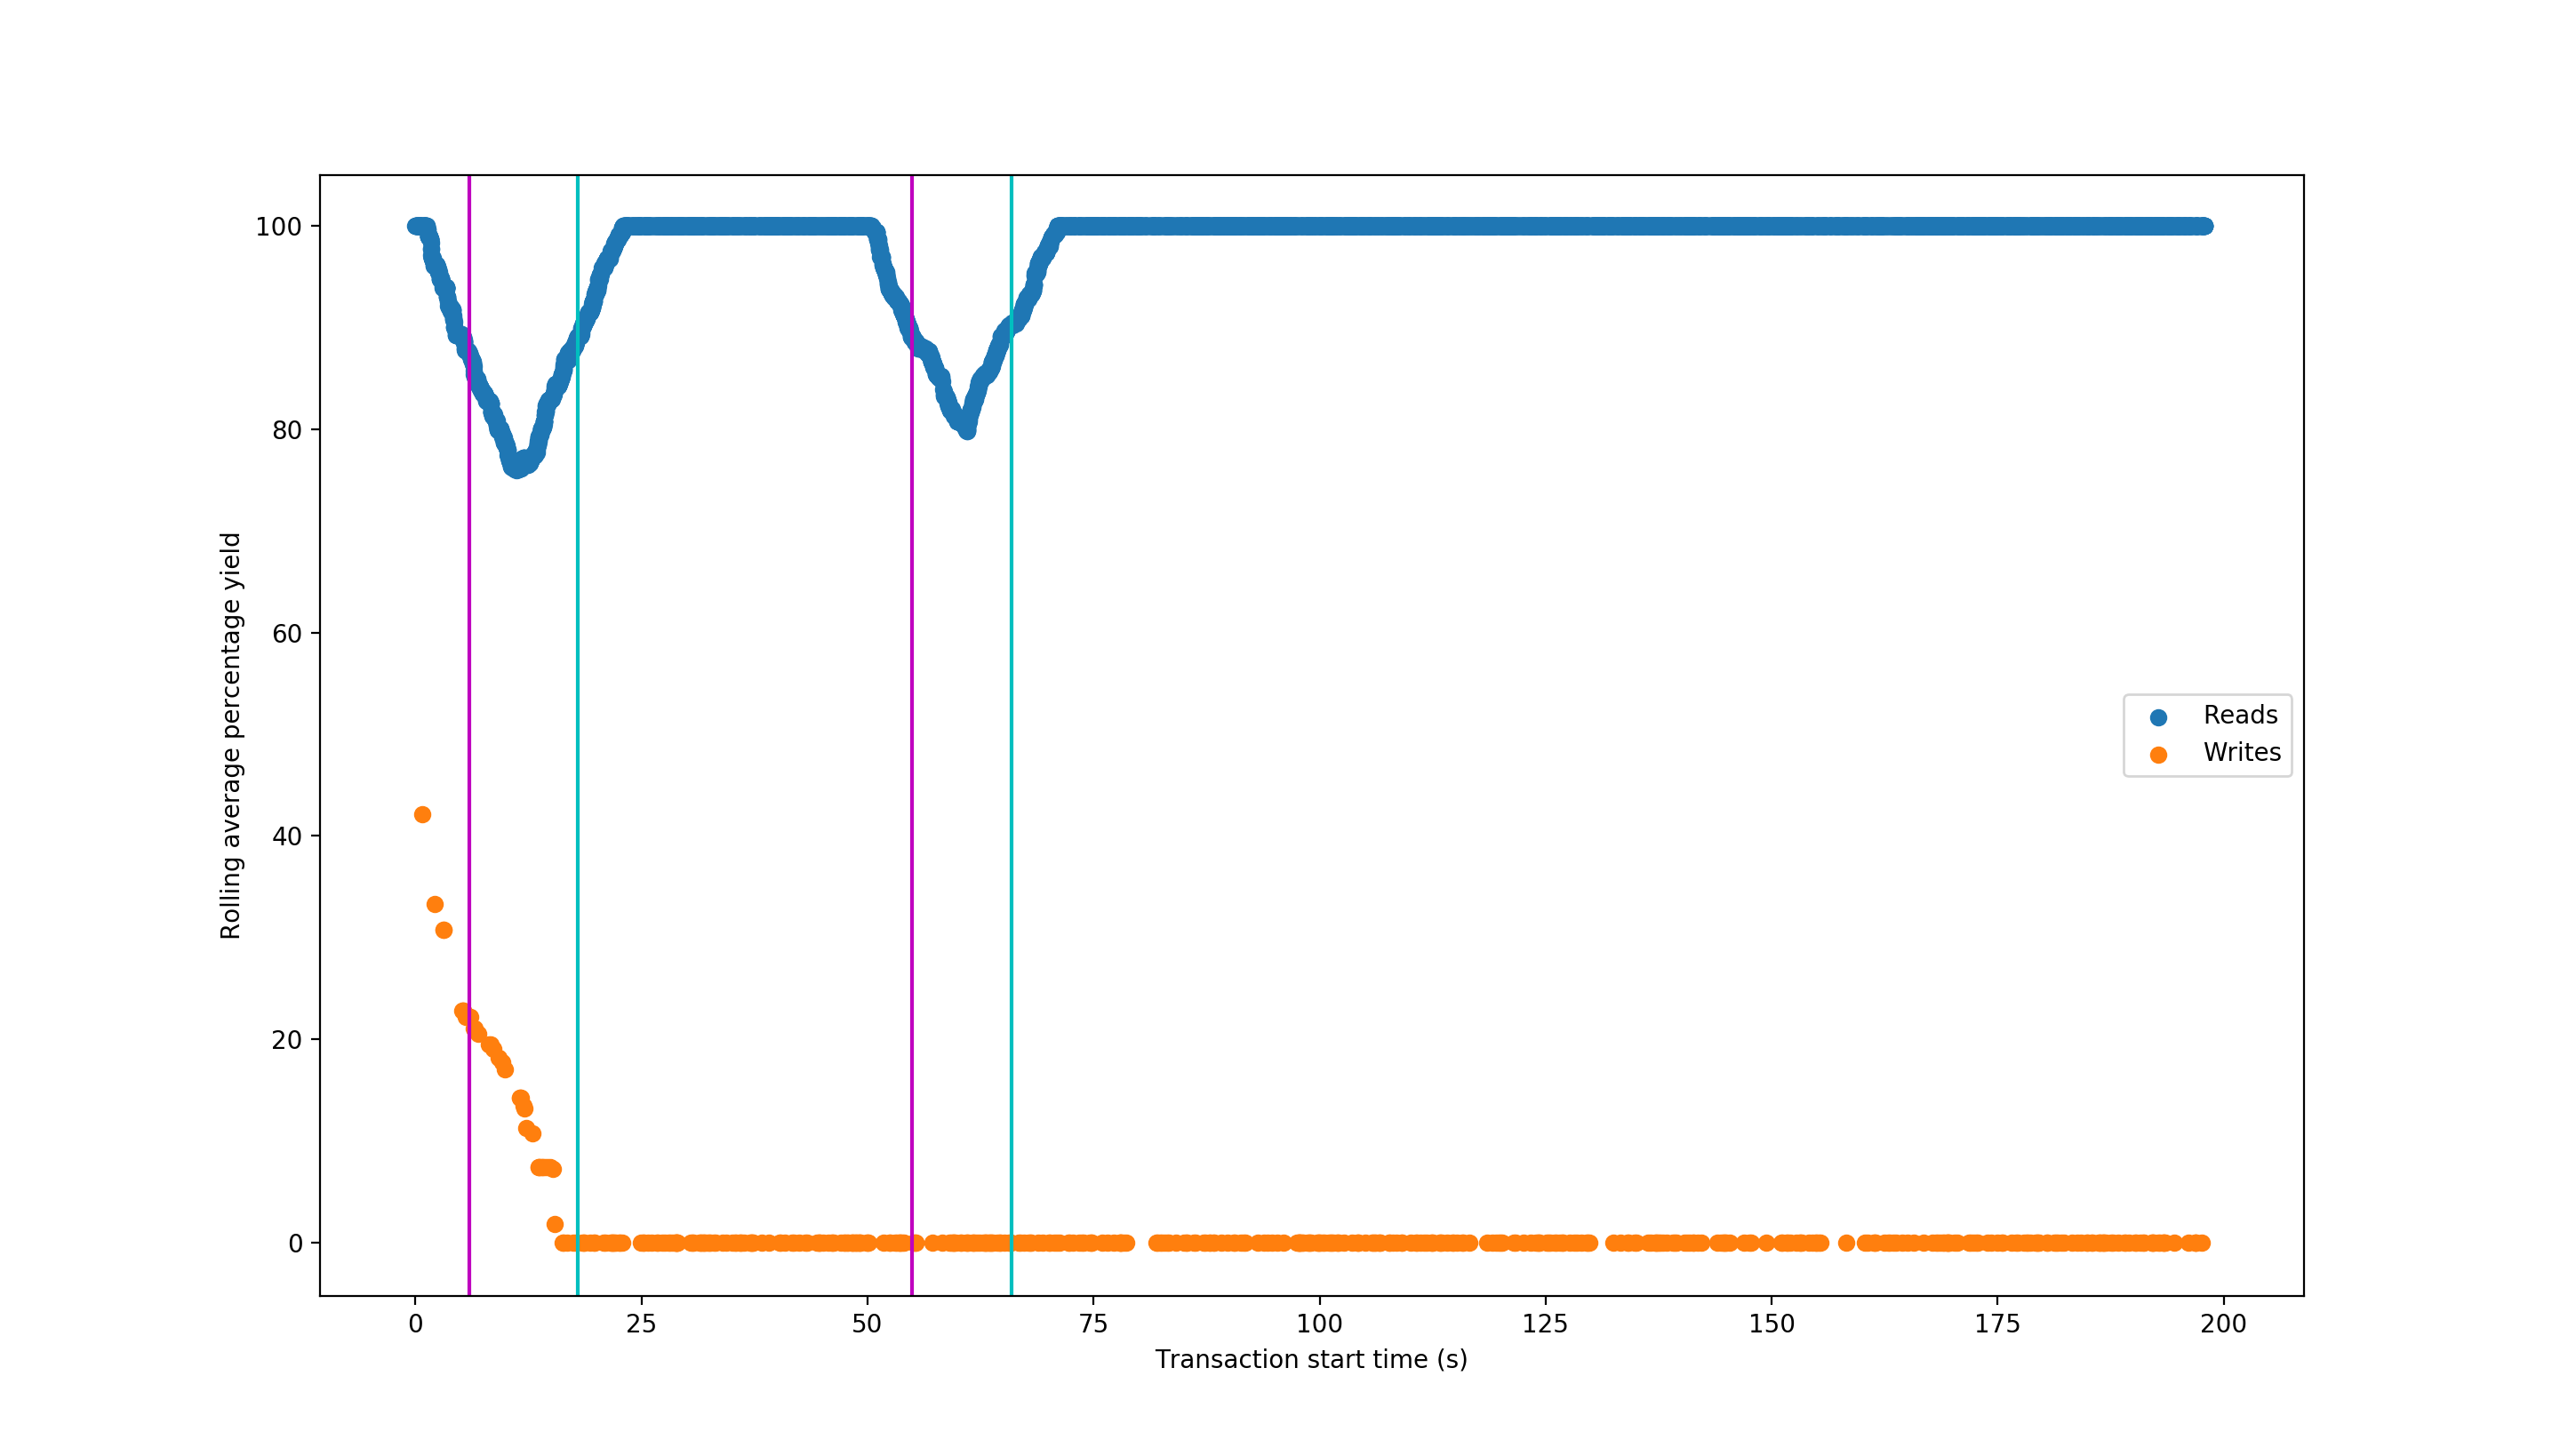
\includegraphics[width=\linewidth]{figs/culprit.png}}
\caption{Rolling average yield over time for a particular test case, with 5 nodes, read quorum size 1, write quorum size 2. Magenta lines indicate single node failures, and cyan lines indicate recoveries. This test was run in an older version of my system, in which nodes failing while assembling quorums would fail permanently. This failure mode occurs if a node fails during a two-phase commit.}
\label{culprit}
\end{figure}

If a node fails permanently, the system may become completely unavailable for some types of transactions, as shown in figure~\ref{culprit}. This failure mode will occur if a node fails permanently during a two-phase commit operation. This is affected by several factors:

\begin{itemize}
\item
My system uses coarse-grained locking: 1 lock for all keys. If there was 1 lock per key, a crash during 2PC would only affect the keys which that particular node was writing to at the time.

\item
Even with fine-grained locking, if $W = N$ (as with strict quorum and $R = 1$), no writes can proceed after any permanent failures. In the general case, if more than $N - W$ nodes fail, the system is unavailable for writes.

\end{itemize}

Google's Spanner has an interesting solution to the limitations of 2PC. Since 2PC requires every member to be available, Spanner has each member be a Paxos group, rather than a single node. This means that, as long as a quorum of nodes in each group is available, two-phase commits can be completed \cite{45855}.


\section{Eventual Consistency Convergence Time}

\begin{table}[h!]
\centering
\renewcommand{\arraystretch}{1.3}
\begin{tabular}{@{} l l l l l l l l l @{}}
\toprule
\bf N & \bf R & \bf W & \bf Transaction Rate & \multicolumn{5}{c}{\bf Convergence Time at Percentile (ms)} \\
& & & & 10th & 50th & 90th & 95th & 99th \\
\hline
3 & 1 & 2 & 50 & 7.66 & 10.63 & 13.7 & 14.74 & 2798.99 \\
& & & 100 & 7.68 & 10.6 & 13.62 & 14.41 & 1867.27 \\
& & & 150 & 7.63 & 10.21 & 13.17 & 14.08 & 15.64 \\
& & & 200 & 7.62 & 10.21 & 13.27 & 14.09 & 16.16 \\
& & & 250 & 7.6 & 10.2 & 13.18 & 14.16 & 215.69 \\
& & & 300 & 7.56 & 10.56 & 13.56 & 14.15 & 1365.01 \\
& & & 350 & 7.65 & 10.58 & 13.7 & 14.99 & 6120.56 \\
\hline
5 & 1 & 3 & 50 & 9.55 & 11.71 & 14.16 & 15.11 & 2618.93 \\
& & & 100 & 9.19 & 11.66 & 14.08 & 15.04 & 18.06 \\
& & & 150 & 9.16 & 11.65 & 14.1 & 15.06 & 17.07 \\
& & & 200 & 9.11 & 11.68 & 14.09 & 15.01 & 17.03 \\
& & & 250 & 9.11 & 11.66 & 14.1 & 15.06 & 2117.5 \\
& & & 300 & 9.19 & 11.69 & 14.07 & 15.0 & 4309.76 \\
& & & 350 & 9.09 & 11.66 & 14.09 & 15.03 & 18.63 \\
\hline
5 & 2 & 3 & 50 & 6.69 & 9.1 & 11.64 & 12.11 & 13.63 \\
& & & 100 & 6.69 & 9.13 & 11.66 & 12.14 & 13.59 \\
& & & 150 & 6.74 & 9.11 & 11.58 & 12.12 & 13.17 \\
& & & 200 & 7.03 & 9.17 & 11.26 & 12.13 & 13.21 \\
& & & 250 & 7.08 & 9.14 & 11.94 & 12.14 & 16.4 \\
& & & 300 & 7.03 & 9.15 & 11.97 & 12.21 & 14.12 \\
& & & 350 & 6.62 & 9.19 & 12.07 & 12.97 & 14.1 \\
\bottomrule
\end{tabular}
\caption{Times for my sloppy quorum system to converge on a strongly consistent state, tested with different quorum sizes and different rates of requests.}
\label{convergencetimes}
\end{table}

These tests are under the same conditions as before, 10 repeats for each set of parameters. Whenever a write transaction is committed or a node writes a new value from background write propagation, a timestamp is logged. The latency for each write transaction is the time from commit until $N - R + 1$ nodes have a copy of the value, so that every read request received after that delay is guarateed to return the most recent value.

Note that this latency is not from the clients point of view. A value is committed before a client response message is sent, and there is latency between a read request being sent and the read being processed by a node.

In my tests, I assumed network latency between any pair of nodes is normally distributed, with mean $10$ ms. With this, if the convergence time is less than $20$ ms at the $n$th percentile, it is more likely than not that $n\%$ of reads will read the latest value (so expect $n / 2 \%$ will read the latest). This assumes the worst case, when a read request is sent immediately after receiving a write response.

At the 99th percentile, my system does not provide consistent convergence time, with spikes most common with $R = 1$. This is due to partitions and node failures. If a partition prevents a coordinator from reaching one or more other nodes, the system cannot converge until the partition recovers. This problem is most likely when $R = 1$; if a single node is unreachable, the system cannot reach the consistent state.

This test does not consider the problem from a client's point of view. If a node has failed completely, it cannot receive the most recent value, but it will not be serving stale values to clients. Spanner provides very high consistency and availability by exploiting this fact; failures are often correlated. For example, suppose an entire data centre goes offline. In that case, all database nodes are unavailable in that data centre, but all application servers in that data centre are also unavailable. If the whole application is unavailable, nobody will notice the database being unavailable \cite{45855}.

These cases are also when eventual consistency is most useful; one data centre could be unavailable and have only stale values, but other data centres can continue serving requests as long as a quorum of nodes is available.

In the common case, convergence times are good. For a few percent of writes, convergence times are less good, due to failures. The stale values due to single-node failures demonstrate the main drawback of $R = 1$.

My system could be modified to provide a bounded staleness guarantee. This would require each node to be aware when values are out-of-date, which could be acheived with a heartbeat. Currently, nodes exchange values when they have update; for bounded staleness, nodes would also need to exchange messages indicating that they have no new changes. If a node has not heard from a critical number of other nodes for some period of time, it must assume its store is out-of-date, and become unavailable for bounded staleness requests.

A bounded staleness with a bound of $10$s of milliseconds should provide at least $95\%$ the yield of normal reads. In practice, this will be higher, since nodes with stale values will be correlated with nodes which are unavailable at any given time. The cost of this is additional network load exchanging heartbeats, which would scale quadratically with the number of nodes.

\section{More Database Nodes}

\begin{figure}[ht]
\centerline{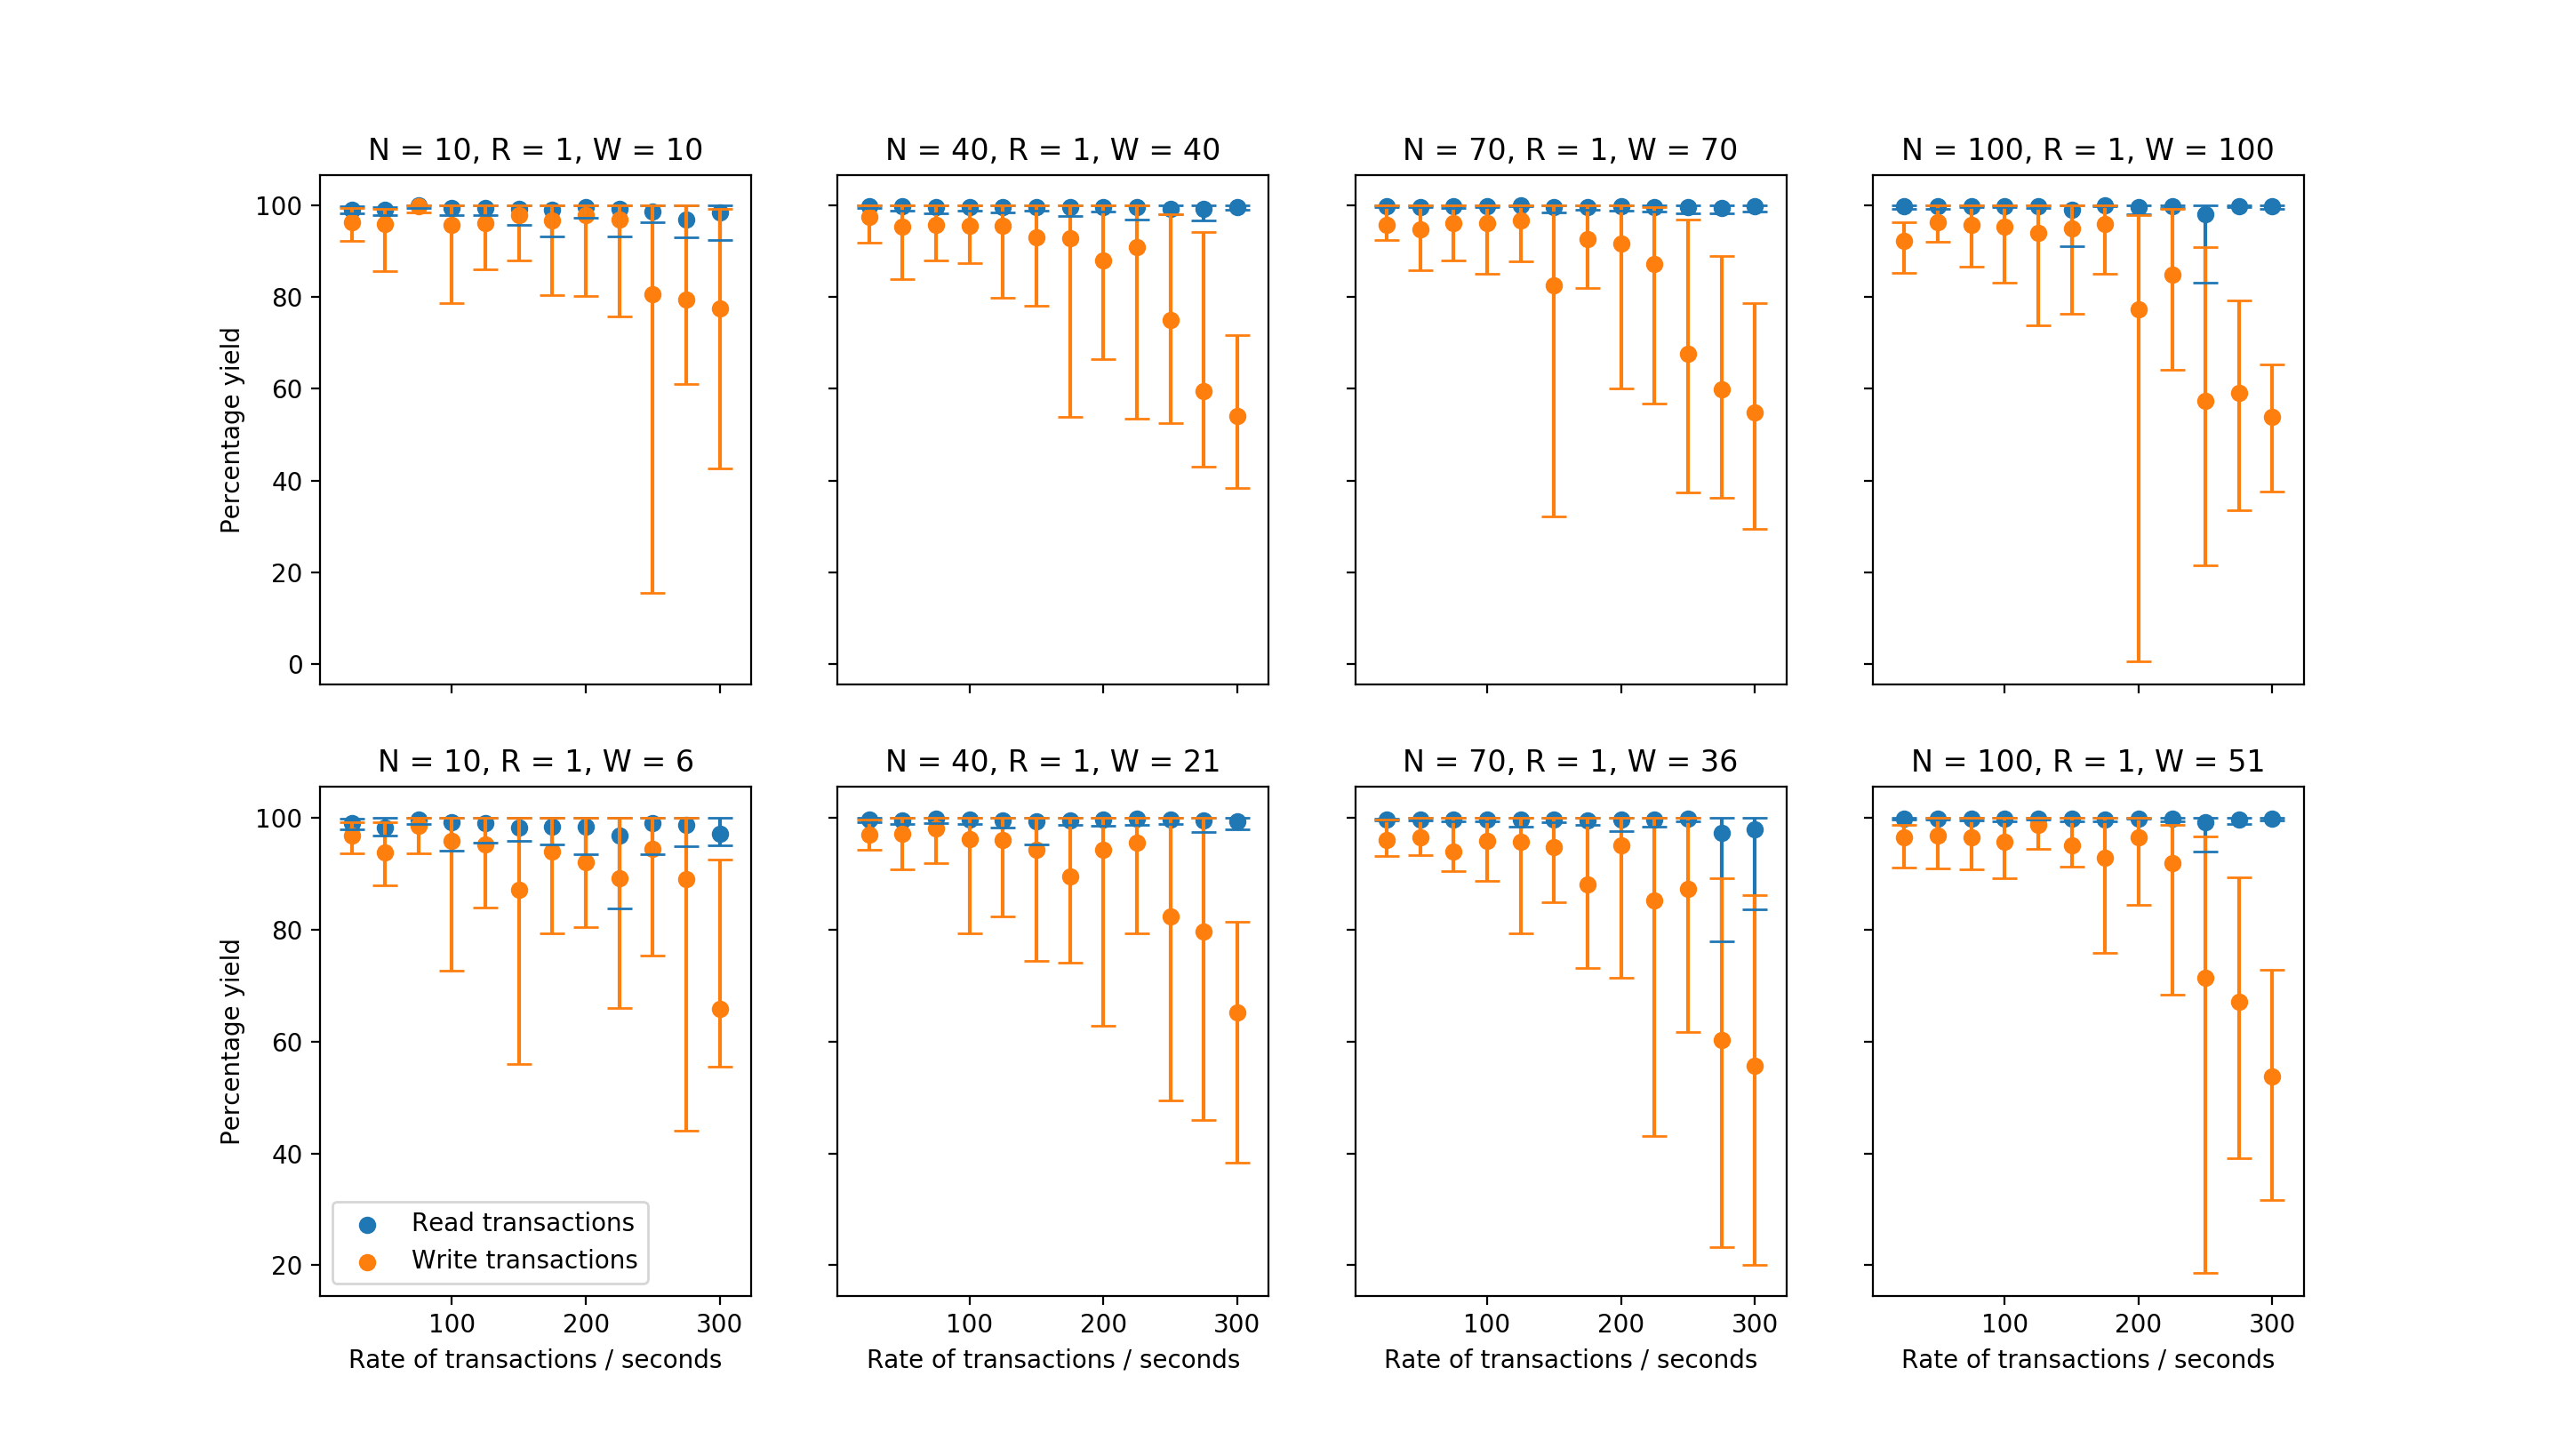
\includegraphics[width=\paperwidth]{figs/big-n-yield.png}}
\caption{TODO}
\label{big-n-yield}
\end{figure}

Figure~\ref{big-n-yield} shows yield for tests with large numbers of nodes (10, 40, 70, 100), testing strict and sloppy quorum for each.

The strict quorum tests appear to be better at higher rates than the previous tests. If a single node fails and clients requests are uniformly distributed between nodes (as they are in all my tests (so far)), the chance of a request reaching a node is greater when the number of nodes is larger. I didn't scale the number of failures to the number of nodes. Partitions will affect more nodes, but failures occur at the same rate.

A failure affecting a small number of nodes affect proportionally less of the system.

\begin{figure}[ht]
\centerline{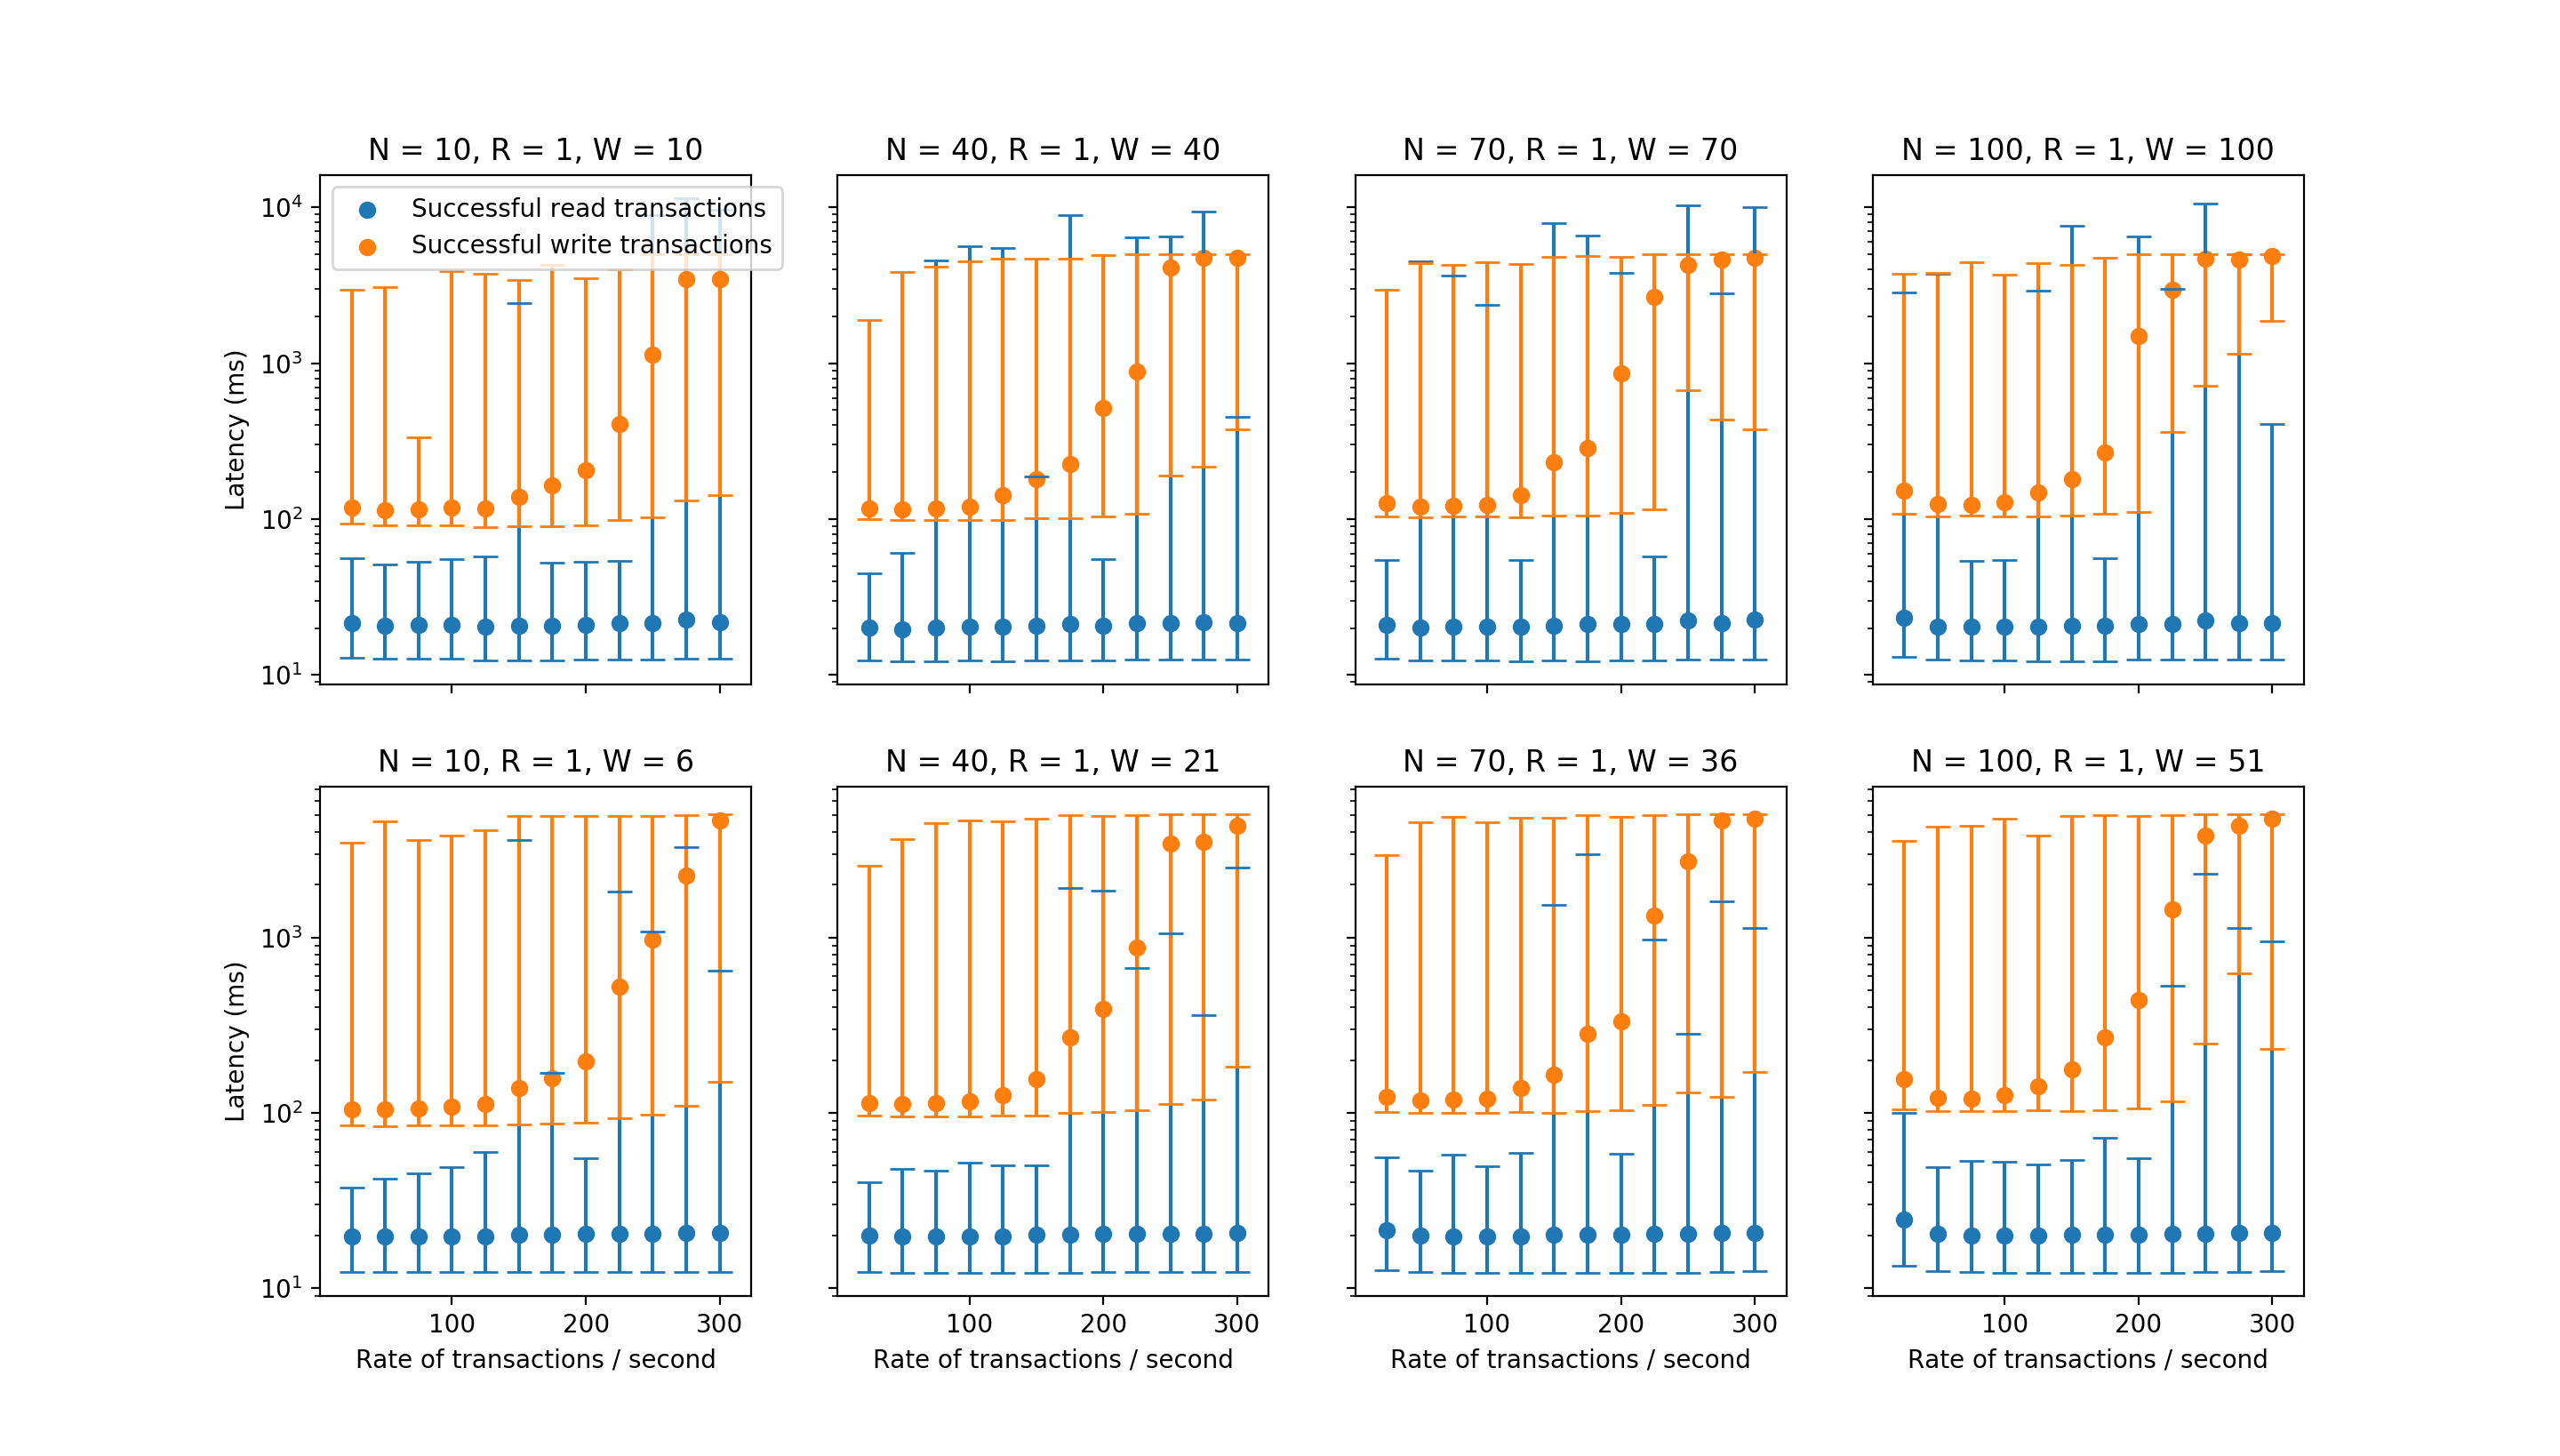
\includegraphics[width=\paperwidth]{figs/big-n-latency.png}}
\caption{TODO}
\label{big-n-latency}
\end{figure}

Figure~\ref{big-n-latency} shows latency of successful transactions in the same set of tests.

As with previous tests where $R = 1$, read latency is very flat. The maximum write latencies are higher: greater chance of a partition affecting a 2PC, which causes the worst case latency when the whole system blocks on a write transaction.

% TODO: reference the appendix
An appendix shows convergence times for tests with large numbers of nodes. As with smaller numbers of nodes, 99th percentile latency has high variance, but 95th percentile is consistent.

95th percentile latency is higher with more nodes. % TODO: justify this claim

% TODO: eval-fig-4, showing a nofail test in detail, justifying why yield is imperfect

% TODO: Comment on how common node failures are \cite{45855}

% TODO: distance matrix, heuristic, test

% TODO: test eventual consistency + monotonic reads \cite{terry2013}

% TODO test with retries

% TODO: test different transaction sizes

\chapter{Conclusions}

% TODO

With hindsight, my design has some notable limitations which were never fixed: global locking and poor multi-tasking. Neither of these issues were fixed, since doing so would require significant refactoring. Had they been identified at an earlier stage, this would not have been a problem.

My system uses global locking, rather separate locks for each key stored. Along with the quorum constraint $W > N/2$, this means that there can never be concurrent write transactions, even when writing to different keys. This means that my system provides external consistency, a stronger guarantee than strong consistency (TODO: refer to explanation), but at the cost of performance.

This limitation amplifies the effect a permanent node failure during 2PC: a single node failure can make the system completely for writes. With fine-grained locking, such a failure would affects to keys which were being modified at the time of failure.

While external consistency is a useful guarantee, global locking is not the best way of providing. Google's Spanner provides external consistency by use of GPS clocks in every data centre. Along with a highly-available private global network, this provides very high availability and a very high level of consistency \cite{45855}. In chapter 1, I claimed that most web applications require partition tolerance, so have to sacrifice either consistency or availability. Spanner demonstrates an exception to this; the trade-off it requires is the cost extensive global infrastructure.

Each database node in my system does a poor job of handling multiple requests simultaneously. The main state in each nodes is implemented as a state machine, with each node always in a single state. For example, a node might be idle, coordinating a read or write transaction, participating in a two-phase commit, etc. This results in requests failing when they could succeed without affecting consistency guarantees. For example, a node participating in a write transaction will not participate in another write transaction's quorum until the first transaction is done. If each transaction writes to a different key, this could be done safely.

To fix this, each node would need to replicate the state machine. Each node would have a set of state machines, indexed by database keys (omitting all keys for which the current state is idle, to minimise memory usage). Assuming no key is accessed too frequently, the system throughput would be limited by hardware, either network bandwidth or disk throughput.

%%%%%%%%%%%%%%%%%%%%%%%%%%%%%%%%%%%%%%%%%%%%%%%%%%%%%%%%%%%%%%%%%%%%%
% the bibliography
\addcontentsline{toc}{chapter}{Bibliography}
\bibliography{refs}

%%%%%%%%%%%%%%%%%%%%%%%%%%%%%%%%%%%%%%%%%%%%%%%%%%%%%%%%%%%%%%%%%%%%%
% the appendices
\appendix

\chapter{Eventual Consistency Convergence Times}

% TODO: introduce the table

\begin{longtable}{@{} l l l l l l l @{}}
\toprule
N & Transaction Rate & \multicolumn{5}{c}{Latency at Percentile (ms)} \\
& & 10th & 50th & 90th & 95th & 99th \\
\hline
\endhead
10 & 50 & 10.68 & 12.66 & 14.97 & 15.75 & 1084.29 \\
& 100 & 10.67 & 12.67 & 14.98 & 15.72 & 1529.33 \\
& 150 & 10.63 & 12.63 & 14.95 & 15.67 & 1372.7 \\
& 200 & 10.65 & 12.65 & 14.93 & 15.69 & 28.86 \\
& 250 & 10.65 & 12.65 & 14.96 & 15.79 & 2233.47 \\
& 300 & 10.71 & 12.72 & 15.01 & 16.06 & 6221.88 \\
& 350 & 10.73 & 12.71 & 15.02 & 16.05 & 5002.91 \\
\hline
\pagebreak[3]
20 & 50 & 11.99 & 13.73 & 15.79 & 16.72 & 3309.74 \\
& 100 & 11.96 & 13.72 & 15.76 & 16.62 & 3573.64 \\
& 150 & 11.9 & 13.7 & 15.69 & 16.12 & 2591.81 \\
& 200 & 11.86 & 13.67 & 15.73 & 16.65 & 1063.04 \\
& 250 & 11.93 & 13.7 & 15.76 & 16.62 & 1464.16 \\
& 300 & 11.99 & 13.73 & 16.0 & 17.08 & 6000.78 \\
& 350 & 11.99 & 13.75 & 15.98 & 17.0 & 5302.29 \\
\hline
\pagebreak[3]
30 & 50 & 12.69 & 14.06 & 16.13 & 17.06 & 3418.1 \\
& 100 & 12.7 & 14.07 & 16.07 & 17.03 & 3260.93 \\
& 150 & 12.7 & 14.05 & 16.04 & 16.93 & 2662.76 \\
& 200 & 12.7 & 14.05 & 16.11 & 17.1 & 4366.88 \\
& 250 & 12.69 & 14.06 & 16.06 & 17.05 & 2728.08 \\
& 300 & 12.71 & 14.07 & 16.05 & 16.99 & 4166.84 \\
& 350 & 12.71 & 14.05 & 16.03 & 16.99 & 4899.38 \\
\hline
\pagebreak[4]
40 & 50 & 13.02 & 14.67 & 16.73 & 17.7 & 3494.65 \\
& 100 & 12.98 & 14.63 & 16.15 & 17.08 & 25.02 \\
& 150 & 12.97 & 14.63 & 16.54 & 17.19 & 2670.02 \\
& 200 & 12.96 & 14.62 & 16.11 & 16.99 & 19.35 \\
& 250 & 12.98 & 14.61 & 16.15 & 17.12 & 6078.53 \\
& 300 & 13.02 & 14.65 & 16.61 & 17.39 & 5121.08 \\
& 350 & 13.02 & 14.62 & 16.14 & 17.09 & 3516.43 \\
\hline
\pagebreak[2]
50 & 50 & 13.62 & 14.94 & 17.02 & 18.18 & 4155.78 \\
& 100 & 13.5 & 14.8 & 16.78 & 17.92 & 3255.07 \\
& 150 & 13.38 & 14.77 & 16.71 & 17.28 & 2528.8 \\
& 200 & 13.29 & 14.76 & 16.65 & 17.16 & 2436.74 \\
& 250 & 13.46 & 14.75 & 16.63 & 17.18 & 1431.5 \\
& 300 & 13.64 & 14.9 & 16.91 & 18.06 & 7022.94 \\
& 350 & 13.29 & 14.98 & 17.06 & 19.89 & 8667.02 \\
\hline
\pagebreak[3]
60 & 50 & 13.77 & 15.08 & 17.21 & 18.86 & 33.38 \\
& 100 & 13.72 & 15.0 & 17.1 & 20.1 & 5926.34 \\
& 150 & 13.71 & 14.97 & 16.88 & 17.66 & 3678.2 \\
& 200 & 13.7 & 14.91 & 16.76 & 17.14 & 21.18 \\
& 250 & 13.72 & 14.97 & 16.74 & 17.24 & 3180.68 \\
& 300 & 13.73 & 15.01 & 16.99 & 17.98 & 5940.44 \\
& 350 & 13.71 & 14.99 & 16.78 & 17.22 & 5260.86 \\
\hline
\pagebreak[3]
70 & 50 & 13.98 & 15.23 & 17.85 & 21.33 & 2065.89 \\
& 100 & 13.84 & 15.08 & 17.07 & 18.02 & 33.41 \\
& 150 & 13.78 & 15.05 & 17.03 & 18.09 & 2807.06 \\
& 200 & 13.79 & 15.03 & 16.99 & 17.91 & 1600.36 \\
& 250 & 13.78 & 15.06 & 16.97 & 17.86 & 2750.67 \\
& 300 & 13.77 & 15.05 & 16.9 & 17.74 & 3694.08 \\
& 350 & 13.89 & 15.07 & 16.96 & 17.25 & 29.88 \\
\hline
\pagebreak[3]
80 & 50 & 14.09 & 15.69 & 18.5 & 23.77 & 1821.92 \\
& 100 & 13.97 & 15.14 & 17.12 & 18.15 & 33.43 \\
& 150 & 13.89 & 15.11 & 17.04 & 17.89 & 26.66 \\
& 200 & 13.88 & 15.12 & 17.07 & 18.01 & 1926.37 \\
& 250 & 13.86 & 15.09 & 17.04 & 17.88 & 3243.03 \\
& 300 & 13.98 & 15.12 & 17.18 & 20.8 & 6638.94 \\
& 350 & 13.99 & 15.11 & 17.02 & 17.75 & 883.9 \\
\hline
\pagebreak[4]
90 & 50 & 14.23 & 15.95 & 19.67 & 27.4 & 5110.88 \\
& 100 & 14.07 & 15.28 & 17.19 & 18.36 & 36.21 \\
& 150 & 14.01 & 15.19 & 17.08 & 18.1 & 932.55 \\
& 200 & 14.01 & 15.2 & 17.08 & 18.08 & 3357.6 \\
& 250 & 14.0 & 15.19 & 17.03 & 17.71 & 30.14 \\
& 300 & 14.03 & 15.16 & 17.06 & 17.91 & 30.14 \\
& 350 & 14.06 & 15.18 & 17.13 & 18.06 & 4455.31 \\
\hline
\pagebreak[3]
100 & 50 & 14.55 & 16.11 & 22.48 & 32.26 & 2450.35 \\
& 100 & 14.19 & 15.66 & 17.34 & 18.87 & 37.96 \\
& 150 & 14.11 & 15.59 & 17.22 & 18.89 & 2755.38 \\
& 200 & 14.09 & 15.29 & 17.06 & 17.9 & 27.9 \\
& 250 & 14.06 & 15.28 & 17.14 & 18.11 & 4806.91 \\
& 300 & 14.1 & 15.25 & 17.15 & 18.24 & 5065.5 \\
& 350 & 14.1 & 15.27 & 17.14 & 18.1 & 3793.45 \\
\bottomrule
\end{longtable}

\chapter{Project Proposal}
%\addcontentsline{toc}{chapter}{Project Proposal}

\setlength{\parindent}{0em}
\addtolength{\parskip}{1ex}

\vfil

\centerline{\Large Computer Science Tripos Part II Project Proposal}
\vspace{0.4in}
\centerline{\Large A Comparison of Consistency Models in Distributed Database Systems}
\vspace{0.4in}
\centerline{\large A.~T.~Bostock, Churchill College}
\vspace{0.3in}
\centerline{\large Originator: A.~T.~Bostock }
\vspace{0.3in}
\centerline{\large 18 October 2018}

\vfil

\vspace{0.2in}

\noindent
{\bf Project Supervisor:} Dr J.~K.~Fawcett
\vspace{0.2in}

\noindent
{\bf Director of Studies:} Dr J.~K.~Fawcett
\vspace{0.2in}
\noindent
 
\noindent
{\bf Project Overseers:} Prof J.~M.~Bacon, Prof R.~J.~Anderson \& Dr A.~S.~Prorok

\vfil
\pagebreak

% Main document

\section*{Introduction}

Distributed database systems are widely used for internet-scale applications. By splitting vulnerabilities across many nodes, we can build systems that continue to function when some nodes are unavailable.

A key limitation for distributed database systems is the CAP theorem: it is impossible to build a system with all 3 of consistency, availability and partition-tolerance. When designing a system, we have to choose the most important properties.

Given the de-centralised nature of the Internet, internet-scale systems need to be partition-tolerant. This means we have a trade-off between consistency and availability. In a critical system, such as a bank's ledger, consistency is most important. In other cases, it may be desirable to sacrifice strong consistency for better availability.

Consider the design of a social networking platform, which allows users to add posts, and serves those posts to other users. For user-experience, it is probably better to serve whatever posts are immediately available, possibly missing the most recent posts, rather than failing to serve any data. It is probably acceptable to have a few seconds delay before a new post is visible to all users.

In this system, we want eventual consistency, where all updates will be available after some time, but not necessarily immediately. This is a weak guarantee. In reality, we probably want new posts to be completely available in less than 1 minute in the vast majority of cases.

My project will explore how quickly an eventually consistent system can reach consensus, and how resource usage differs between a strongly consistent system and an eventually consistent system.

\section*{Work to Be Done}

I will build a strongly consistent, distributed key-value store based on quorum assembly. The system will store data on a fixed number of nodes, with all data replicated across every node. This will include:

\begin{itemize}
  \item
  Quorum assembly: requiring a minimum number of nodes be involved in every read and write transaction, and each node involved in a transaction be locked. This ensures serialisability of transactions, by preventing any transaction from accessing data concurrently with another transaction modifying the same data.

  \item
  As part of quorum assembly, an atomic commit protocol is needed, to assure that values are either written to a whole write quorum, or not written at all. For this, I will implement the two-phase commit protocol (2PC).

  \item
  To track which nodes have stale data, I will build a vector clock system.

\end{itemize}

The system will be designed in a modular fashion, so that each component can be replaced to make a new version of the system with different characteristics.

I will build, as a module, a sloppy quorum system. Using this, I will build an eventually consistent variant of the database system.

I will build a test framework to test and evaluate the systems. This should simulate a network of nodes using one machine. It should be able to:

\begin{itemize}
  \item
  Simulate an unreliable network, including random latency and packet loss.

  \item
  Simulate failure of individual nodes.

  \item
  Randomly generate streams of requests, and send them to the system. Requests generated should simulate those from a social network application: many read transactions, a smaller (but still large) number of transactions adding a new key (and value), and a small number of transactions modifying or removing an existing key. Requests should be sent randomly, at a given average rate (following a Poisson distribution).

  %\item
  % The system should also be able to send any given sequence of requests. For example, to measure time to reach consistency in an eventually consistent system, I could send a write transaction, and then repeatedly send read transactions to each node, to measure the time to reach consistency.

  \item
  Record data for each request sent: request data, request timestamp, and response data and timestamp (if a response is received).

\end{itemize}

Alongside the metrics reported by my test framework, I can use profiling tools to measure resource usage by different parts of the system.

I will evaluate the strongly-consistent and eventually-consistent variants of the system using some or all of the following metrics:

\begin{itemize}
  \item
  System throughput: average time taken to process a large number of requests.

  \item
  For the eventually consistent version, time taken to reach consistency.

  \item
  CPU and memory usage of each node (and average across all nodes).

\end{itemize}

Each of those can be measured for different numbers of nodes, different quorum (or sloppy quorum) sizes, different rates of transactions, different network conditions, and different scenarios involving node failures.

I will implement the project using Go. Go is a fast, compiled language, making it ideal for low-level systems projects. It is also statically typed, and uses garbage collection, so it is safer and easier to work with than C, a commonly-used language for systems programming. Go also has good support for concurrent programming, which will be helpful for building a test framework, using concurrent components to simulate a distributed system.

\subsection*{Success Criteria}

This project will be considered a success if I have done all of the following:

\begin{itemize}
  \item
  Built a strongly consistent distributed key-value store. This system must, when tested with 5 nodes:

  \begin{itemize}
    \item
    Support get and put operations. \verb|put(key, value)| must either successfully store the given key and value, or error. \verb|get(key)| must either return the most recently put value for the given key, or error.

    \item
    Continue to function properly after 2 nodes have failed.

  \end{itemize}

  \item
  Built a variant of that system which is eventually consistent.

  \item
  Evaluated the throughput of each system when using different numbers of nodes, and different rates of transactions.

  \item
  Evaluated the time taken for a value written to the eventually consistent system to be completely available, under different network conditions.

\end{itemize}

\subsection*{Extensions}

\begin{itemize}
  \item
  Implement three-phase commit (3PC), and evaluate the performance of the system when using 3PC compared to 2PC.

  \item
  Explore and evaluate methods for optimising the sloppy quorum system to minimise the time to reach consistency.

  \item
  Explore different data structures for storing data on each node, and evaluate their performance, including how significant the choice of data structure is compared to the design of the distributed components of the system.

\end{itemize}

\section*{Starting Point}

I have some experience using Go, having previously used it for a personal project (implementing a regular expression processor).

I have previously studied distributed systems in the IB course Concurrent and Distributed Systems.

\section*{Resources Required}

I will use my personal laptop (2017 MacBook Pro). I accept full responsibility for this machine and I have made contingency plans to protect myself against hardware and/or software failure.

 I will use git and GitHub for version control, Backblaze for cloud backup, and an external disk for additional weekly backups.

I will use Go to implement my project, so I will use its open-source compiler and tools.

In case of failure of my machine, I can restore from one of the backups, and continue working by logging onto a remote private server on Digital Ocean (on which I can install Go tools and my preferred editor, Kakoune), using an MCS machine. This should allow me to continue working with minimal interruption.

\section*{Timetable}

\subsection*{18 Oct - 31 Oct}
Produce a detailed design of the system, presented as a document which can be used later when writing the preparation and implementation chapters of the dissertation.

\textbf{Milestone:} Specification document completed, and approved by supervisor.


\subsection*{1 Nov - 14 Nov}
Build a basic test framework, so that I can use it to test the distributed database system.

\textbf{Milestone:} A basic test framework complete, with support for running multiple nodes, generating test transactions, and verifying that system output is as expected.


\subsection*{15 Nov - 28 Nov}
Implement quorum assembly, including 2PC.

\textbf{Milestone:} All tests passing for the quorum assembly module.


\subsection*{29 Nov - 12 Dec}
Build a strongly consistent key-value store, based on quorum assembly.

\textbf{Milestone:} Key-value store implemented, all tests passing.


\subsection*{13 Dec - 26 Dec}
Slack time / work on extensions.

\textbf{Milestone:} All tests passing for the strongly consistent database.


\subsection*{27 Dec - 9 Jan}
No work around Christmas time.

\subsection*{10 Jan - 23 Jan}
Write a progress report.

Prepare a presentation.

\textbf{Milestone:} Progress report submitted (by 12:00 1 February).

\textbf{Milestone:} Presentation prepared.

\subsection*{24 Jan - 6 Feb}

Extend the database system to use a sloppy quorum system, to provide eventual consistency.

\textbf{Milestone:} Presentation delivered.

\textbf{Milestone:} All tests passing for the sloppy quorum version.


\subsection*{7 Feb - 20 Feb}

Extend the testing framework to simulate different conditions and provide system metrics, as required for evaluation.

Evaluate the strongly consistent and eventually consistent versions of the system.

Write a draft evaluation chapter for the dissertation.

\textbf{Milestone:} Draft evaluation chapter written, and sent to supervisor for feedback.


\subsection*{21 Feb - 6 Mar}

Write an outline dissertation, including important figures and a summary of each section's content.

\textbf{Milestone:} Outline dissertation complete, and sent to supervisor for feedback.


\subsection*{7 Mar - 20 Mar}

Slack time / work on extensions.

\textbf{Milestone:} All success criteria met.


\subsection*{21 Mar - 3 Apr}

Write dissertation: preparation and implementation chapters.

\textbf{Milestone:} Preparation and implementation chapters complete, and sent to supervisor for feedback.


\subsection*{4 Apt - 17 Apr}

Write dissertation: all remaining chapters.

Make changes to implementation and evaluation chapters based on feedback.

\textbf{Milestone:} Dissertation complete, and sent to supervisor/DoS for feedback.


\subsection*{18 Apr - 1 May}

Make changes to dissertation based on feedback.

Slack time / work on extensions.

\textbf{Milestone:} Dissertation complete, including changes based on feedback.


\subsection*{2 May - 15 May}

Slack time.

\textbf{Milestone:} Dissertation submitted (by 12:00 17 May).




\end{document}
